\chapter{CosmoLIME}
All the pieces of the puzzle have finally fallen into place and we are now finally in the position to properly introduce \textsc{CosmoLIME} and explain its inner workings in detail. We have covered both the pros and cons of the static approach to emulation in cosmology: we discussed that, while on one hand providing ready-made emulators can greatly accelerate parameter inference pipelines, on the other as soon as a strict set of conditions is violated the ready-made emulator can no longer be used, thus declaring the failure of the out-of-the-box approach. We argued that this issue can be tackled with a new design paradigm: instead of providing already trained emulators a possible new approach consists of assembling a framework in which everyone can build their own custom emulator, tailored to their particular needs. By automating the emulator's training procedure it becomes possible to significantly reduce the human time needed to obtain a functional model: ideally this new software should be able to accept minimal user inputs (which models to try on which data, the target accuracy, etc.), which can be achieved by standardizing the training and testing procedures.

We also discussed why it makes sense to focus on power spectra emulation - more in general why indirect approaches to likelihood, based on comparing some observed variables and theoretical predictions, are advantageous; this is important, because it guides the design of this framework towards the approximation of \emph{functions} rather than \emph{distributions}, allowing us to use tools from the ``easy'' side of machine learning. This is important, because even though a likelihood and its power spectrum may be mathematically and physically equivalent learning them can require different machine learning tools.

Speaking of these tools we summarized the main results about supervised learning with a special focus on functional regression, as well as the main machine learning techniques needed to perform regression in practice (models, accuracy metrics, train/test split, etc.); these results provide us with the low-level ingredients needed to solve the high-level problem of power spectra emulation to accelerate parameter inference.

The combinations of all these mathematical, physical and statistical results culminates in the design principles with which \textsc{CosmoLIME} has been designed: \textsc{CosmoLIME} is a model-agnostic, self-training, machine learning-based software framework that can learn to emulate arbitrary likelihood in a fully automated way - by learning the functional form of the power spectrum equivalent to the likelihood at hand.

We can finally begin our discussing how taking all these factors into account translates into the design of the inner workings of \textsc{CosmoLIME}.

\section{Design Principles}
\subsection{Software Hierarchy}\label{subsec:software_hierarchy}
% bella figura tikz

% abbiamo tutti gli elementi per automatizzare il processo di creazione di un emulator. Recap degli step necessari: dataset + training + test. Pertanto ci servono dei blocchi di data generation e di model training (facoltativo il preprocessing), piò una classe manager. Principio di design del software = modularità, cioè ogni blocco può essere definito e usato in modo indipendente, ma ovviamente la vera forza di cosmolime sta nel lasciare che la classe mega faccia queste cose da sola

% recap non solo dei passaggi che servono per il training in generale di TUTTI gli emulator (utile per introdurre i 3 blocchi di base: generator, preprocessing, optimizer, più il manager e la questione delle componenti), ma anche delle features che deve avere cosmolime. Di queste ultime non ha senso rifare la discussione nel primo capitolo; basta spiegare come siano soddisfatte dal blocco corrispondente (ad esempio optimizer accetta modelli arbitrari supponendo che la classe fornita dall'utente abbia un metodo di training, poi si occupa lui di fornire gli iperparametri del modello, i dati, il testing dei risultati, eccetera).

We now possess all the elements needed to automate the process of creating a functioning emulator; in particular since the procedure to train an emulator is in principle always the same we can use it to define the basic building blocks of \textsc{CosmoLIME}. 
We know that building an emulator is a three-step process:
\begin{enumerate}
    \item Generate a dataset via simulation;
    \item Train a (set of) machine learning predictor(s);
    \item Test the result with metrics based on realistic inference pipelines.
\end{enumerate} % AGGIUNGERE FIGURA TIKZ DI QUESTI 3 PASSAGGI?
The only things that may change when training different emulators are the training/test dataset and the machine learning models of choice, but that e.g. the data must be generated and then fed to the model is fixed. Since implementing an emulator requires the interchange between these two phases (data generators and model training) it makes sense to create a sub-block for each one of them. We also need classes to deal with optional preprocessing transformations (if needed) and a pair of them to manage all the different blocks. For this reason \textsc{CosmoLIME} consists of 5 main classes:
\begin{enumerate}
    \item The \texttt{generator} classes accepts as input a \texttt{python} function that computes exact cosmological parameters-power spectrum values (e.g. by wrapping Boltzmann solvers); at the same time it deals with other issues, such as the caching of generated samples.
    \item The \texttt{preprocessing} class optionally transforms the data generated by \texttt{generator} using the transformations provided by the user, with default options available - while offering utility features, like \texttt{generator}.
    \item The \texttt{optimizer} class takes the preprocessed generated data and trains the user provided machine learning models, dealing with the problem of hyperparameter optimization automatically - which is often the most tedious and time-consuming part of training machine learning models. Once again this class provides nice utilities, like the logging/pretty printing of the results.
    \item The \texttt{component} class creates and manages an instance of \texttt{preprocessing} and of \texttt{optimizer}, while also implementing the logic needed for ``dynamic'' training: while \texttt{optimizer} expects and trains over a single, fixed dataset, \texttt{component} is capable of \emph{requesting} new data samples and tasking \texttt{optimizer} with a new run of the training algorithm if the performance of the previous run is deemed unsatisfactory. More on this later on.
    \item The \texttt{emulator} class manages all of the above. In particular it ensures the user does not have to manually instantiate all the needed classes, and allows them to provide a single input dictionary containing all the requested models etc. that are to be tested by the software.
\end{enumerate}
We remark that all of these classes have been designed both with independence and interoperability in mind; this means that all of them can be used independently (which can be useful to e.g. tinker manually with some parts of the emulator-building process), but that the user can simply provide some input arguments to the emulator ``super-class'' and let it instantiate and manage everything.

A quick summary of the above can be represented with a picture.
\begin{figure}[H] % prova a imitare il disegno di Luca
    \centering
    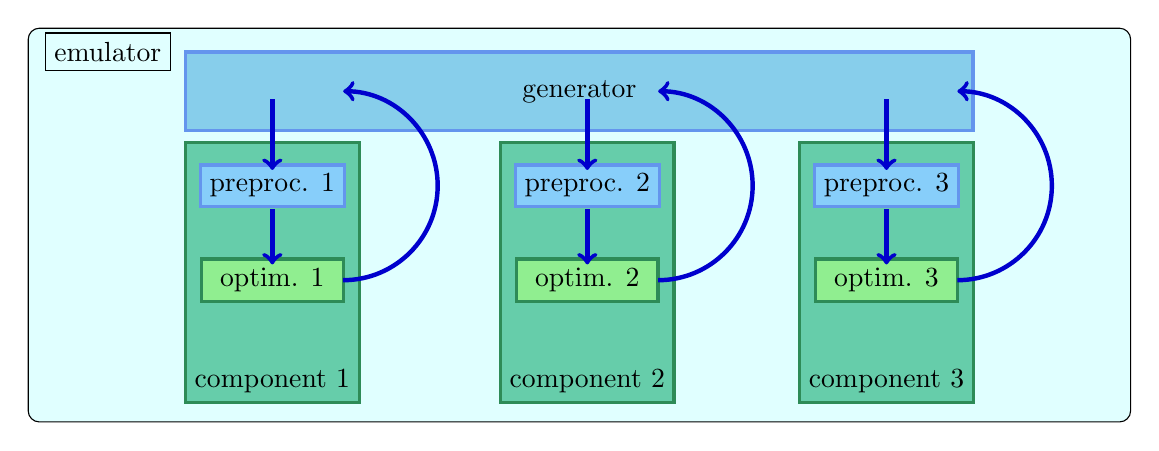
\begin{tikzpicture}[
    gennode/.style={rectangle, draw=CornflowerBlue, fill=SkyBlue, very thick, minimum height=10mm, minimum width=100mm},
    ppnode/.style={rectangle, draw=CornflowerBlue, fill=LightSkyBlue, very thick, minimum size=5mm},
    optnode/.style={rectangle, draw=SeaGreen, fill=LightGreen, very thick, minimum width=18mm},
    compnode/.style={rectangle, draw=SeaGreen, fill=MediumAquamarine, very thick, minimum height=30mm, minimum width=10mm, text height=30mm}, % red!60 e red!5
    ] % recupera nodi e frecce da overleaf tikz tutorial
      % \draw[rounded corners, black] (0, 0) rectangle (14, 5) node[pos=.1] {\texttt{emulator}}; % pos=.1: al 10% del viaggio da (0,0) a (14,5) aggiungi un nodo testuale
      % \node[draw, rounded corners, black] (0, 0) rectangle (14, 5) {}; % non gli piace
      \draw[rounded corners, black, fill=LightCyan] (0, 0) rectangle (14, 5) {};
      \node[draw] at (1.01, 4.7) {emulator}; % aggiungi il testo sopra direttamente^
      
      \node[gennode] (maintopic) at (7, 4.2) {generator}; % specificarne la posizione?
      
      \node[compnode] at (3.1, 1.9) {component 1};
      \node[ppnode] at (3.1, 3) {preproc. 1};
      \node[optnode] at (3.1, 1.8){optim. 1};
      \draw[ultra thick, ->, color=MediumBlue] (3.1, 4.1) -- (3.1, 3.2);
      \draw[ultra thick, ->, color=MediumBlue] (3.1, 2.7) -- (3.1, 2.0);
      \draw[ultra thick, ->, color=MediumBlue] (4, 1.8) arc (-90:90:1.2);
      
      \node[compnode] at (7.1, 1.9) {component 2};
      \node[ppnode] at (7.1, 3) {preproc. 2};
      \node[optnode] at (7.1, 1.8){optim. 2};
      \draw[ultra thick, ->, color=MediumBlue] (7.1, 4.1) -- (7.1, 3.2);
      \draw[ultra thick, ->, color=MediumBlue] (7.1, 2.7) -- (7.1, 2.0);
      \draw[ultra thick, ->, color=MediumBlue] (8, 1.8) arc (-90:90:1.2);

      \node[compnode] at (10.9, 1.9) {component 3};
      \node[ppnode] at (10.9, 3) {preproc. 3};
      \node[optnode] at (10.9, 1.8){optim. 3};
      \draw[ultra thick, ->, color=MediumBlue] (10.9, 4.1) -- (10.9, 3.2);
      \draw[ultra thick, ->, color=MediumBlue] (10.9, 2.7) -- (10.9, 2.0);
      \draw[ultra thick, ->, color=MediumBlue] (11.8, 1.8) arc (-90:90:1.2);
      
    \end{tikzpicture}
    \caption{Schematic representation of \textsc{CosmoLIME}.}
    \label{fig:cosmolime_schematics}
\end{figure}

Notice that in fig. \ref{fig:cosmolime_schematics} we have one generator, but several components. The reason for this is that codes like \texttt{camb} can generate multiple derived quantities (power spectra, predictions of observables, etc.) starting from the same set of parameter values, and we may want to train separate machine learning models on these different parts of the dataset; more on this later on. In general what we have is a generator that produces several streams of data in parallel, which are stored and fed sequentially to each component. The component currently in training takes the generated data, performs the preprocessing, then looks for the best model hyperparameters using the optimizer; if needed it will request more data and try again. The emulator class oversees this whole procedure.

\subsection{Common Design Rules}\label{subsec:common_design_rules}
To conclude this introduction to \textsc{CosmoLIME}'s technical explanation we describe a few mandatory design rules that are shared by all of \textsc{CosmoLIME}'s blocks.

\paragraph{Data Representation in Memory}
An important property of \textsc{CosmoLIME} is the \emph{shape of the data} it deals with. 
\textsc{CosmoLIME} performs functional regression to learn the mapping between cosmological parameters and power spectra; this means mapping a vector input (parameters) to a vector output (spectra predictions). We can therefore stack observations vertically, thus organizing our dataset into a pair of matrices i.e. rectangular arrays of real numbers. For this reason \textsc{CosmoLIME} represents the dataset in memory using mostly rectangular \texttt{numpy} arrays, which is a common choice for this type of problems.
Usually these arrays are small enough to comfortably fit into memory: dealing with tens of thousands of rows made of tens of real numbers is not an issue for modern computers; for this reason \textsc{CosmoLIME} always makes the assumption that a ``big data'' approach (i.e. offloading the matrices to disk and only load in memory a fraction at a time) is not necessary.\footnote{A big data approach is not impossible, just not implemented in the current version of \textsc{CosmoLIME} as it has not yet been deemed necessary.}
In general going forward we keep in mind that \emph{\textsc{CosmoLIME} datasets are rectangular arrays of real numbers}, i.e. matrices where the rows represent the observations and the columns the different variables.

\paragraph{Block independence}
As explained above \textsc{CosmoLIME} consists of several blocks, all of which work in tandem to assemble an emulator using an automated, standardized algorithm; the automated algorithm to assemble an emulator is the intended use-case of \textsc{CosmoLIME}. 
In order to ensure that different usages are also possible each block is designed to be not just collaborative with the others, but also fully independent; this means that each block can be manually instantiated, accessed, and used, while also being capable of working in harmony with the others. This is useful for testing purposes, but can also be relevant if we want to disassemble the main class after training (for example we may want to use the same trained preprocessing block to perform different analyses, which means we may want to be able to discard the generator and model attached to that block).
These two scenarios (blocks used on their own or together) are both allowed as long as we ensure that the classes are both human-friendly and computer-friendly, so that both a human and \textsc{CosmoLIME}'s automated procedures can easily use them; to achieve this there are both ``manual'' and ``automatic'' modes to use the methods in each class. This basically means that we can use the available methods interactively, i.e. by manually modifying the class' internal state as needed, or automatically, i.e. by fixing all the relevant arguments once and for all during object initialization, then calling its method with no arguments. This second approach is taken by the manager classes: they automatically instantiate the needed classes with fixed internal parameters and then use them always in the same way; a human instead can take them apart, use their methods with new values for the internal parameters, and so on.

\paragraph{Support For External \texttt{python} Data Science Packages}
\texttt{python} offers many great packages to extend its data analysis and machine learning capabilities; examples include \texttt{numpy}, \texttt{scikit-learn}, \texttt{pytorch}, and so on. In order to exploit these remarkable packages \textsc{CosmoLIME} has been designed with this in mind, using the ``open slot'' approach to ensure inter-package compatibility. For example the \texttt{optimizer} class is able to accept an arbitrary user-provided model; as long as the associated class contains a \texttt{.train()} method it can be used by \texttt{optimizer}, because its internal algorithm leaves an ``open slot'' to be filled with any class, then calls this object's train method. This level of abstraction (which consists of writing code where some elements are left as generic as possible and are then filled by the user) is shared by all software blocks; in this way all the great available packages can be used with minimal effort, requiring at most a wrapper to satisfy \textsc{CosmoLIME}'s consistency requirements. Were this not the case we would need to reinvent the wheel too many times, because we would need e.g. to re-implement common machine learning algorithms from scratch.

\paragraph{}
Finally we can now dive into the detailed explanation of exactly how these pieces work and communicate.


\section{Generator}
% importante il discorso che possiamo avere dati infiniti (potenzialmente), ergo non c'è solo da usare modelli più sofisticati (compromessi eccetera)

% ha senso mettere anche i dettagli tecnici del codice, ad esempio che possiamo scegliere un numero iniziale di samples da generare così come quanti aggiungerne ad ogni giro.

% Importante il discorso di alternanza fra generazione e miglioramento modello (parametro di ogni quante epoche generare) così come quello del caching delle componenti non attualmente in uso; tutto questo da illustrare con gli esempi di camb

% prova a vedere che succede usando meno dati, ad esempio se cosmolime decide di prenderne altri (non c'è bisogno di rieseguire la funzione, basta definire un sampling che sia un indexing statico del numero di righe richieste dove l'offset è dato dal seed*num iniziale, così scorro senza ripetizioni)

\subsection{Simulating Data}\label{subsec:simulating_data}
The most important part of any machine learning application is the dataset; without good enough and plentiful enough data the world's most sophisticated algorithm will still perform badly.\footnote{Many people in the machine learning community underestimate how often the same algorithm performs much better after new data is acquired or e.g. a better preprocessing pipeline is employed; this ``gamification'' of machine learning means that often people scramble to achieve the best score over some fixed dataset by changing the algorithm instead of acting upon the dataset itself.} An interesting aspect of \textsc{CosmoLIME} is related to this crucial point, as its treatment of data samples is quite unusual.

In most machine learning application the data is fixed, which means that the acquisition of new samples is not possible. For example many popular big data models require the assembling of huge datasets, which is an expensive and time-consuming procedure; therefore once the dataset has been obtained people would rather optimize the performance of the model rather than invest more time and money in the sampling of new data points.
Another common occurrence is that of noisy data; for example if the points in the dataset have been obtained by experimentally measuring some quantity (like e.g. in many scientific machine learning applications) then there always are spurious contributions of some sort afflicting the dataset. For this reason even in basic regression problems one always models the process as the sum of two contributions: a deterministic part (the actual model we care about) and a stochastic part (the noise term we would like to eliminate but cannot). Even though statistics can help deal with the ever-present noise (via preprocessing or noise modelling) it can never be completely removed.

Probably the most interesting feature of emulating cosmological power spectra from a machine learning perspective is that these two common limitations (fixed, noisy datasets) do not apply; to see why this is true let us compare the generic regression problem in machine learning with the one pertaining to \textsc{CosmoLIME}.
The typical situation where one applies regression is when an \emph{unknown} function must be learned from data; due to the fact that the mapping is unknown we can only measure $(x, f(x))$ pairs and use them to infer the overall shape of $f$. Furthermore if the $(x, f(x))$ pairs are obtained with an imperfect procedure (e.g. noisy measurements, suboptimal sampling) their quality constrains how accurately we can approximate $f$ with its $\hat{f}$ representation.
But when dealing with power spectra the mapping $f$ is \emph{known}; the point of emulation is to accelerate the evaluation of a known function, not learning an unknown one - therefore since $f$ is known it becomes possible to select an arbitrary set of points $\{x_n\}$ and evaluate the corresponding function values $\{f(x_n)\}$. This procedure has two important implications: in this machine learning problem we can generate as much data as we want, and the obtained samples will have perfect accuracy,\footnote{At least in principle; since $f$ is usually a complex function what is typically done is to evaluate it using numerical techniques, which may lead to inaccuracies.} since no noise sources are present.

Indeed notice that access to data with arbitrary quality and of arbitrary number is in general the main difference between the emulation task and a generic regression problem; the remaining elements (e.g. the numerical techniques) are instead shared between these tasks. This crucial difference hinges on whether $f$ is known (and just to be accelerated), as in the specific task of function emulation, or whether $f$ is unknown (and therefore to be actually discovered, at least approximately), as in the most general regression problem.

To recap: instead of approximating the relation between two fixed, noisy datasets we can generate as much noise-free data pairs as needed. Therefore when designing \textsc{CosmoLIME} we do not want a class that accepts a prebuilt dataset and passes it to the next layer; what we want instead is to implement a block capable of automatically sampling data points. This block's user provided input, therefore, is not a fixed dataset, but rather a \texttt{python} function capable of computing $f(x)$ when fed with $x$. 

These considerations steer the design process towards defining the \texttt{generator} block so that it performs the following actions:
\begin{enumerate}
    \item It generates new data samples when asked;
    \item It passes the obtained datasets to the appropriate parts of the emulator;
    \item Finally it optionally caches data, either in memory or on disk. Saving on disk is useful to avoid having to start from scratch in the event that unexpected errors cause the program to suddenly fail; saving in memory is needed to comply with the ``parallel generation, sequential training'' approach when dealing with multi-component datasets (see next sections).
\end{enumerate}
Let us discuss these points in more detail.

\subsection{Sampling Strategies}\label{subsec:sampling_strategies}
% griglia deterministica, prendere parametri a caso, non ci esprimiamo perché qui l'utente ha modo di sfruttare eventuali prior suoi (nel senso di problem knowledge ma anche letteralmente riguardo come campionare parametri)
As said above in the case of \textsc{CosmoLIME} the user can afford the luxury of not having to supervise the process of obtaining the dataset; instead they can simply give \textsc{CosmoLIME} the means to automatically assemble the dataset as needed. When discussing the \texttt{component} class below we will describe the logic used by \textsc{CosmoLIME} to decide more data are needed; for now we simply need to understand how \texttt{generator} can satisfy the request of simulating new points, when asked. To describe how this is implemented in \textsc{CosmoLIME} it pays off to approach the problem from a more general point of view.

Let us suppose we need to sample a function $f$ by evaluating it in some arbitrarily chosen points $\{x_n\}$, so that an output dataset $\{f(x_n)\}$ can be obtained. We want to use the $\{(x_n, f(x_n))\}$ pairs to learn an approximation of $f$, which naturally leads to the following question: how should the points $x_i$ be chosen to ensure the most accurate learned representation of $f$ possible? If we could sample infinitely many points we could achieve perfect approximation accuracy, but clearly this is impossible; ideally we want to choose the $x_n$ in strategic regions of parameter space, so that a good machine learning algorithm may be able to interpolate the missing parts of $f$ accurately enough.

Several strategies are possible to sample the $x_i$ points:
\paragraph{Grid Sampling}
The simplest possible approach is to define a grid of linearly spaced points, and use it to define the $\{(x_n)\}$ sequence. In the case of parameters with bounded values (i.e. parameters only defined in a finite interval) this is trivial; in the case of parameters that can be arbitrarily small or large (or even just defined in very large intervals) we need to select a minimum and maximum values in order to construct this grid. For example in the case of a function mapping 1D spaces after defining $x_{\text{min}}$ and $x_{\text{max}}$ (either arbitrarily or due to the physics of the problem) and how many points to sample we can compute each element of the $\{x_n\}$ sequence as follows:
\begin{equation*}
    x_n = x_0 + n\Delta x = x_0+n\frac{x_{N-1}-x_0}{N-1} = x_\text{min} + n\frac{x_{\text{max}}-x_{\text{min}}}{N-1}, \ \ n\in [0, N-1]
\end{equation*}
from which it follows that in this notation $x_0 = x_{\text{min}}$ and $ x_{N-1} = x_{\text{max}}$.

This approach to choose the $\{x_n\}$ sequence reflects a lack of preference for any region in the $\mathcal{X}$ space (i.e. the vector space the $x_n$'s belong to). Picking this sampling strategy is reasonable when we want to express the belief that no $x$ values are more important than others, or when we lack knowledge about the function's behaviour in $\mathcal{X}$. In general this sampling strategy represents not committing to any spot in particular, treating them all equally; in Bayesian terms we may state that this strategy is equivalent to an \emph{uninformative prior}, i.e. we do not express information that would allow to give different weights to different regions of $\mathcal{X}$ space.

% svantaggio gaussiana
This approach is indeed useful when the user knows that all regions of $\mathcal{X}$ should be sampled uniformly and deterministically, or if they're unsure about the shape of $f$ and want to pick the ``safe'' option; and yet this approach can be inefficient. Imagine for example that the target function $f$ is almost constant in region $\mathcal{X}_1$, while quickly varying in region $\mathcal{X}_2$; a simple example of this is a Gaussian, that is almost zero outside the tails and quickly rises to its maximum value once we start walking towards the peak. Now in this case having an equal number of points in $\mathcal{X}_1$ and $\mathcal{X}_2$ is inefficient: too many points in $\mathcal{X}_1$ is a waste because few samples are needed to accurately summarize $f$'s behaviour here, while too few points in $\mathcal{X}_2$ may cause the model to fail in the task of accurately capturing the shape of the function (at most the model can learn a sort of local average, while missing the high frequency details contained in $f$). This potential issue can be mitigated by increasing $N$: with a huge number of points in the dataset each part of $\mathcal{X}$ is bound to be adequately represented. In practice, though, $N$ cannot be too large, as we often have a limited computational budget: computing each $f(x_n)$ can have a non-negligible cost, so that large enough values of $N$ can be impractical. For this reason it makes sense to explore other sampling strategies, in particular strategies that are intrinsically asymmetric in the sense that they prefer certain regions of $\mathcal{X}$ over the others.

\paragraph{Uniform Random Sampling}
% uniform distribution
Another possible sampling strategy consists in selecting the $x_n$ \emph{randomly} in $\mathcal{X}$, then computing the corresponding $f(x_n)$ values. This can be helpful because with limited values of $N$ can introduce some asymmetry in the sampling procedure. Considering the previous example, where the target function $f$ varies slowly in $\mathcal{X}_1$ and quickly in $\mathcal{X}_2$, sampling the $x_n$ points randomly makes it possible that more point will happen to be in $\mathcal{X}_2$ rather than in $\mathcal{X}_1$. 

To better appreciate this result imagine that the overall behaviour of this function $f$ is unknown - that is, we know how to compute $f(x)$ for any $x$ but we don't know e.g. how $f(x)$ varies with $x$, and so on. Let us also imagine that in this situation $N$ cannot be too large due to computational budget constraints, and that the grid approach results in a model of $f$ with unsatisfactory performance. Even if we do not know about $\mathcal{X}_1$ and $\mathcal{X}_2$ by switching to a random sampling approach with a bit of luck we may stumble upon the efficient asymmetric distribution of the $\{x_n\}$ sequence in $\mathcal{X}$ space.

Assuming we lack prior knowledge about $f$'s behaviour in different regions of $\mathcal{X}$ the most reasonable distribution to use is the \emph{uniform} one, as we have no way of committing to a preference for e.g. $\mathcal{X}_2$ over $\mathcal{X}_1$; but this sampling strategy can lead to inefficiencies, too. Indeed unless $N$ is quite small the observed distributions of points will quickly converge to the uniform one they're sampled from, i.e. the sampled sequence $\{x_n\}$ will become symmetric with respect to the different regions of $\mathcal{X}$. Since this convergence is relatively quick this means that even for $N$ values that are not particularly big we recover the previous grid-based case, i.e. a sequence of points that fails to implement the asymmetry needed to increase the efficiency under budget constraints.

In order to achieve the desired asymmetry we may therefore restrict ourselves to small values of $N$; in this case the population distribution can actually significantly differ from uniform, and therefore be asymmetric in $\mathcal{X}$. The problem with this approach is that by staying away from convergence we cannot predict much about the resulting distribution, which basically means that whether the output sequence is good or not is left to luck. Assuming we can try to sample the population of points several times this may not be an issue: even if the first attempt failed maybe after 10 the resulting distribution efficiently captures $f$. In this case we will have sampled $10N$ points instead of $N$; if $N$ is small enough that $10N$ is not too expensive but e.g. $10^5N$ would be needed to ensure success with grid sampling then this uniformly random strategy can be successful. Unless we are in this sweet spot, though, it makes sense to implement a truly asymmetric sampling strategy.

% uniform prior: democratico, ma nel limite riproduce quanto sopra nel senso che nel limite è troppo simmetrico. Inoltre si basa sulla fortuna

\paragraph{Nonuniform Prior Sampling}
% custom sampling distribution
If prior knowledge about $f$ is available how to design more efficient samplers becomes almost obvious. Sticking to the grid approach, for example, we can ditch the linearly spaced grid in favor of one that is finer in ``hotter'' regions (those with more ``activity'') and coarser in the ``cold'' ones.
Another possibility is to use random sampling from a \emph{non-uniform} distribution: as we saw switching to a stochastic sampling strategy makes it possible to achieve a good $\{x_n\}$ sequence with much fewer points, but whether this possibility is actually realized in practice is unpredictable and therefore requires some luck. We remark that it becomes possible to decrease the amount of luck if a nonuniform distribution is employed: indeed if we know that $\mathcal{X}_2$ requires more points than $\mathcal{X}_1$ we can design the sampling distribution in such a way that points from $\mathcal{X}_2$ are more likely, and so on. In this sense a nonuniform distribution introduces the needed asymmetry in the same way as the nonuniform grid, but as mentioned multiple time can potentially reach the results with less points (with the price to pay being that we cannot know beforehand whether the next run will actually be successful).

\subsubsection{The Problem of Specifying Prior Knowledge}\label{subsubsec:prior_knowledge_generator}
% coarse grid, slightly finer grid, until the points are numerous and packed close to each other (per riciclare il parametro seed nel caso deterministico)
% tre passaggi
The discussion in the previous section outlines an important fact: \emph{it is best to avoid fully automating the sampling procedure}. What we mean is that, since each sampling strategy has pros and cons, the most efficient way to decide where to evaluate e.g. a power spectrum depends on the specific problem at hand, and on how the user decides to deal with it. For this reason we believe that the decision of the sampling strategy is best left to the user; not only that, but the user must also write a wrapper to their Boltzmann codes of choice. 

The \texttt{generator} class therefore expects a \texttt{python} function from the user; this function must do the following:
\begin{enumerate}
    \item Accept a \texttt{size} and a \texttt{seed} argument;
    \item Sample \texttt{size} number of points $\{x_n\}$ using the sampling strategy of choice, using the \texttt{seed} parameter as seed;
    \item Compute and return the $\{f(x_n)\}$ sequence by feeding the each $x_n$ to the exact code of choice.
\end{enumerate}
% SCHEMATIC REPRESENTATION USING TIKZ? TUTTE QUESTE FIGURE MI POSSONO TORNARE UTILI PER LA PRESENTAZIONE E RENDEREBBERO LEGITTIMA LA PRESENZA DI UN INDICE DELLE FIGURE

Defining this function is the only nontrivial piece of user-written code required by \textsc{CosmoLIME}, as the rest simply consists of specifying some arguments like which model is to be optimized. Indeed by using a user-provided function defined with these rules the \texttt{generator} can generate as many points as requested by \texttt{component}; the \texttt{seed} parameter can be used to ensure reproducibility and that the points sampled every time the \texttt{generator} is called are actually different.

\paragraph{What About Deterministic Sampling Strategies?}
Having \texttt{generator} rely on a \texttt{seed} parameter makes it seem that \textsc{CosmoLIME} is unfairly biased towards stochastic sampling strategies, but we the user can easily write the required function in such a way to comply with the \texttt{seed} argument requirements even assuming a deterministic sampling strategy. As we will see later \textsc{CosmoLIME} uses the \texttt{seed} parameter to increase the size of the training data in the event of unsatisfactory model performance by setting \texttt{seed} equal to the index of the current epoch. This means that the algorithm starts with a seed equal to 0, then if \texttt{component} determines that more data is needed it will ask \texttt{generator} to produce more using \texttt{seed = 1}, and so on; in the case of stochastic samplers this means sampling the distribution multiple times to collect more points. This means that the role of the \texttt{seed} parameters is simply controlling the size of the final dataset. Therefore if we write the above function with \texttt{seed} controlling the coarseness of the grid we can ensure that \textsc{CosmoLIME} will work as expected; for example with \texttt{seed = 0} the grid may be very coarse, while with \texttt{seed = 5} the grid is much finer. 
Due to this it seems that in the case of deterministic samplers the \texttt{size} and \texttt{seed} parameters overlap; after all if increasing the \texttt{seed} is supposed to produce a finer grid it must then imply a larger number of samples in the dataset, therefore overruling the number of samples to be generated specified by \texttt{size}. Furthermore this seems to be a problem, because a 10 times finer grid has 10 times as many points, resulting in the request of generating an ever-increasing number of points instead of the fixed value specified by \texttt{size}.

These issues are actually easily tackled in practice: since generating data is a cumulative process (i.e. the new samples are put in the same dataset as the old ones) we can create a finer grid by adding a fixed number of points, instead of starting from scratch with a larger number of points to produce. A possible way to achieve this with a fixed \texttt{size} and increasing \texttt{seed} is to generate linearly spaced grids offset by an amount depending on \texttt{seed}; in this way we can surely increase the density of points in our grid while at the same time keeping the number of generated points per epoch fixed.

We remark that other approaches are possible, and that we need not concern ourselves with details about the role of \texttt{size} and \texttt{seed}, as those will be explained later in more detail; the point of this paragraph is simply that the design philosophy behind \texttt{generator} is flexible enough to accomodate for arbitrary sampling procedures.

\subsection{Data Components: Parallel Generation, Sequential Training}\label{subsec:data_components_generator}
% mettere da parte gli altri dati: parallel generation, sequential training
Boltzmann solvers like \texttt{camb} \cite{camb} work by allowing the user to fix the detail of the cosmology (model, parameter values, etc.), then computing predictions for several observable quantities; we call these separate outputs \emph{components}. Dealing with multiple components is useful because by observing the corresponding quantities in independent experiments we have multiple ways of constraining the cosmology, considering their common source. For this reason it makes sense to have separate machine learning predictors, one for each component i.e. one to replace each separate theoretical prediction. 
An important property of softwares like \texttt{camb} is that predictions come in bulk: the software outputs \emph{all} of these components in a single batch; this has the advantage of allowing for \emph{parallel data generation}, in the sense that a single call to \texttt{camb} returns the input-output pair of values for all the observables at the same time. In theory this would allow \textsc{CosmoLIME} to also train the model associated to each component at the same time: as the new data arrive each part of them is streamed to the appropriate component, which then proceeds to train its respective model at the same time. The problem with this is that training a machine learning model can be quite intensive: depending on the complexity of the model all the available computer resources may be required. In order to avoid reaching obvious bottlenecks \textsc{CosmoLIME} was designed in such a way that data are generated in parallel, but the corresponding component models are trained in sequence; we will describe later how this works in practice.\footnote{As stated it is wiser to train one model at a time; hence what \textsc{CosmoLIME} does instead is to optionally use the approach discussed in the next sections to train several versions of the same model in parallel. Possible extensions of this ``partial parallelization'' will be discussed later on.}

For now we remark that this ``parallel data generation, sequential training'' approach means that \textsc{CosmoLIME} alternates between a data generation phase and a model training one, with the property that during the data generation all component datasets are sampled, while during the training one only one model at a time. In order to comply with this algorithm \texttt{generator} has a way to hold onto data that will be used later: every time it is requested to generate data for e.g. component 1 it generates data for \emph{all} components; then it returns the data for component 1 and stores the remaining component datasets in memory or on disk, to be used when the training phase switches to the other components' models. This \emph{component caching} functionality is a core part of \texttt{generator}; in particular its component data generation method simply wraps the method used to call the user-provided function with this separation and caching of components.

\subsection{Other \texttt{generator} Features}
% salvare su disco, accettare parametri... roba pallosa e più o meno intuibile da quanto sopra
The remaining arguments when initializing \texttt{generator} can be used to customize the saving behaviour; for example in the case of datasets that require expensive computations one can enable the saving or offloading of the other components' datasets to disk, and even though this slows down \textsc{CosmoLIME} it can prevent the need to face long waits multiple times in the case that the software suddenly stops due to an error. Other options can be used to set hyperparameters in the user-provided function, and to allow for the saving and loading of datasets in separate locations: if for example a dataset is already available (e.g. because the user has already simulated data with the same function) it can be loaded and used as a starting point, so that \textsc{CosmoLIME} does not have to generate data completely from scratch. There are also options to avoid overwiting this ``prior'' dataset, so that previous analyses can be kept separate.

Finally notice that by default datasets are saved to or loaded from disk using either the \texttt{.npy}, \texttt{.npz} or compressed \texttt{.npz} format. As stated above we are performing regression, which means that our datasets are comprised simply of matrices: for example the input is a matrix whose rows represent different ``observations'' (i.e. different values for the set of input cosmological parameters), while the columns represent different parameters altogether. Since we are dealing with ``rectangular'' datasets of real number these datasets are efficiently represented as \texttt{numpy} arrays; we therefore also save them to disk using \texttt{numpy}'s methods.


\section{Preprocessing}
\begin{comment}
- i tecnicismi tipo nan remover e constant features remover?
- log: riduci il dynamic range tipo cosmopower quando possibile (features positive), ma almeno in output a volte ha senso anche analiticamente (ad es. il log di una MVN è solo la parte di forma quadratica) - direi che questo è più un esempio per contestualizzare il log, qua si parla di preprocessing, schiacciare gli ordini di grandezza mi sembra più pertinente
- media a zero e varianza a 1, utile ad es con le NN ma non con gli alberi. In alternativa: min e max a 0 e 1, eccetera
- whitening: media a zero e covarianza identica (cioè identità non solo sulla diagonale ma ovunque, tolgo le correlazioni fra variabili, cioè tengo solo le dipendenze statistiche di ordine superiore)
- super whitening: cross correlation fra input e output, rendo identica la cross correlation (una specie di super covarianza) fra input e output. In questo modo considero una dipendenza statistica "semplificata", che tenga solo gli ordini superiori. Questo viene fatto con la procedura del prof. Chiarire sia perché questa procedura funzioni sia più in generale a che serva.
- altro? Rivedi il codice
- (prima) discussione generale di trasformazioni solo di input o output, o quelle accoppiate, congiunte
\end{comment}
\subsection{Standardized Preprocessing Interface}
The most important part of any machine learning application is the dataset; the second one is the preprocessing, and the last one is the model. The reason for this is that if the training data's quality is poor not even the world's most advanced model can turn those samples into accurate predictions. Having covered how we can generate and manage an arbitrary number of arbitrarily accurate samples we now turn to the problem of designing a standardized interface for arbitrary data preprocessing transformations.
% differenza con dataset: anche se resta possible avere trasformazioni completamente fatte dall'utente stavolta possiamo offrire trasformazioni di default ragionevoli, in quanto trasformazioni universali sicuramente esistono - a differenza di "dati universali", che non esistono in quanto evidentemente dipendenti dal problema in questione.
The problem of choosing a (set of) preprocessing transformer(s) is similar to that of choosing the data generation/sampling procedure, in the sense that the user should decide one of several possible approaches depending on the problem at hand. As we saw we can interpret the choice of the generation algorithm as reflecting some sort of prior knowledge on the problem; the same is true for data preprocessing, because data preprocessing transformations must be chosen according to the special characteristics of the problem and of the model of choice.
In the case of \texttt{generator} this is a necessity: there is no universal way to generate data because they clearly depend on the physics of the relevant situation; and yet this is no longer true in the case of preprocessing. Indeed there exist ``universal'' transformations of the data, in the sense that some transformations that are useful in a large class of problems (for example standardizing the dataset's mean and variance can help numerically stabilize a neural network's training); for this reason \texttt{preprocessing} can be asked to implement one of \textsc{CosmoLIME}'s default transformers (do note that custom made transformers can still be used, of course).

The \texttt{preprocessing} class in \textsc{CosmoLIME} works in a similar way as \texttt{generator}: the user provides either a custom or default (set of) transformer(s), then \texttt{preprocessing} fits its hyperparameters to the data (if any; see below). Once this is done \texttt{preprocessing} can be used as any other \texttt{python} function, i.e. it can take any pair of input/output datasets and return the transformed versions. Notice that if an inverse transformation is available a method computing it is contained in the corresponding class, too; not all of them have it because some transformations discard informations and are therefore irreversible.
% FIGURA SCHEMATICA IN TIKZ?

\paragraph{Joint Transformations}
Most preprocessing transformations are applied to only the input or the output matrix; for example as we will see below in order to ensure that the input dataset's features have zero mean it suffices to subtract their averages, without the need to involve the output dataset.

Some transformations, though, are \emph{joint}: they involve both the input and the output dataset (for example \texttt{NaNJointRemover}; see below). For this reason the \texttt{preprocessing} module has internal subclasses that correctly interface with any transformation depending on whether it is joint or not. Therefore two informations must be specified by the user should they want to provide a custom transformer: the mathematical transformation and whether or not \texttt{preprocessing} should consider it a joint input/output transformation.

\subsection{Default Transformers}\label{subsec:default_transformers}
% listona in paragrafi?
% ConstantFeaturesRemover NaNJointRemover LogTransformer Log1pTransformer StandardScaler Whitening (vari schemi, cita paper pca, più complesso: joint decorrelation...)
Several prebuilt transformers are available in the \texttt{preprocessing} module for the user to choose from; let us review them. 
\subsubsection{Recommended Transformers}
\textsc{CosmoLIME}'s default option for preprocessing consists of the sequence of the following transformations.\footnote{Of course the default option is not mandatory: the user can choose a different set of transformations, or even disable preprocessing entirely.}

\paragraph{\texttt{NaNJointRemover} Transformer}
A typical use-case of \textsc{CosmoLIME} consists in generating data using \texttt{camb}. This means that the generator will pass a set of cosmological parameters values to \texttt{camb}, which will respond with the theoretical prediction of some observable conditioned on those values for the cosmological parameters. For technical reasons certain input values lead to outputs containing \texttt{NaN} (not a number) values; of course it usually is impossible to know beforehand which numerical values ``corrupt'' the predictions, and we can only compute predictions and a posterior ban the inputs that led to the empty outputs.

Some machine learning algorithms and preprocessing transformations are capable of dealing with \texttt{NaN} inputs, either by ignoring them or by classifying them separately (e.g. some decision trees-based models can do this distinction); but considering that the vast majority of machine learning models will fail if \texttt{NaN}s are not removed it is wiser to discard them from the dataset. This is an example of a joint transformer: we want to remove rows from the input matrix depending on the output one.
The \texttt{NaNJointRemover} transformer solves this problem by obtaining a logical mask which marks which rows in the output matrix contain at least one \texttt{NaN}; this mask is then used to drop the coupled rows from both matrices, i.e. the rows in both matrices which share the same index. 

For obvious reasons the logical mask used to flag and remove bad rows is recomputed every time a new dataset is presented.
We also remark that the discarded rows are not saved anywhere, therefore this transformation is irreversible, hence why it is given an identity inverse transform.

\paragraph{\texttt{ConstantFeaturesRemover} Transformer}
Sometimes the user-provided function passed to \texttt{generator} can have redundant outputs%. 
% For example when computing the predicted luminosity distances associated to a grid of redshift values the distance at $z=0$ will always be zero, by definition; since this value is the same irrespective of the employed cosmology one output feature (i.e. matrix column) will be constant and equal to zero. % non ne sono più così sicuro...
; for example the generation code may produce a constant feature i.e. a constant column; due to this all rows share one element, which means all but one are redundant.
The user can account for this by slightly tweaking their code, but in the event they forget about it or do not want to deal with this correction themselves it makes sense to check for constant features. 
The \texttt{ConstantFeaturesRemover} performs this automated check and correction; it does so by computing a logical mask to flag columns whose elements all share the same value. This is achieved in a vectorized fashion by assigning \texttt{True} to the columns (if any) whose elements are all equal to e.g. the first one. If the mask produced this way flags any column (either in the input or the output) those columns are removed from the respective matrix, similarly to the previous transformer. The main difference is that this transformation is invertible: this class remembers the index of the discarded column and its only value, so that it the original matrix may be easily restored. To achieve this two arrays (positions and values) are stored in the transformer.

\paragraph{\texttt{StandardScaler} Transformer}
As discussed in section \ref{subsec:nn} a simple preprocessing transformation that often results in improved performance (especially in the case of some models, like e.g. neural networks) is \emph{feature standardization}; standardizing the features means rescaling each variable i.e. each column according to one of several possible rules. For example a common choice consists in rescaling the variables so that they all have zero mean and unit variance. To achieve this it suffices to compute the mean and standard deviation along rows, i.e. the mean and std obtained using the elements of all the rows; we can then subtract the mean array from each row, then divide by the std array, resulting in a matrix whose rows have zero mean and unit variance.
Using numpy this is easily achieved using a vectorized approach: \texttt{(x - x.mean(axis = 0))/x.std(axis = 0)}.

This transformation is invertible, too: by remembering the mean and std arrays of the original dataset and inverting the algebric operation given above the original matrices can be reconstructed exactly. This in turn requires that this transformer, too, must hold an internal state, whose value is to be learned by fitting the data.

As a final remark we note that this transformer is not custom made, as are the other two; it actually comes with no modifications from the \texttt{scikit-learn} package. This is consistent with one of \textsc{CosmoLIME}'s design principles, namely support for external \texttt{python} packages; this is just one example of how beneficial the consequences of \textsc{CosmoLIME}'s design philosophy can be in practice.

\paragraph{Default Transformer}
The default preprocessing transformation consists of the previous three transformers, in the same order as above. The first two don't really have disadvantages and should always be utilized, as they basically check for imperfect or suboptimal \texttt{generator} outputs, that the user did not preemptively account for. The last one is a less obvious choice: even though feature standardization often helps or is innocuous at most (for example in the case of decision trees), experience tells that sometimes standardizing the features can actually impede convergence speed or accuracy, as it often is a nontrivial modification of the data distribution. In this cases or in the event the user is unsure the scaling transformation can be disabled easily enough; since the ``helpful or harmless'' cases are more common we decided to leave it in the default transformer anyway.

\subsubsection{Optional Transformers}
\textsc{CosmoLIME} currently includes other preprocessing transformations; since these do not always improve the training procedure they are left to the user's discretion. 
A few examples are reported here.
% log, log1p, whitening + io decorrelation
\paragraph{\texttt{LogTransformer}}
There are several situations where applying a logarithm to the input or output features can greatly aid an inference pipeline. For example since Gaussian likelihoods are very common in cosmology a standard procedure is to compute the \emph{log-likelihood} instead of the original likelihood; in this way it becomes possible to only deal with the quadratic form. This is exactly what softwares like \textsc{CosmoPower} do; instead of computing the power spectra directly they predict their \emph{logarithms}.

Applying a logarithm transform in situations like the previous example is a natural choice due to the mathematical properties of the problem at hands; even when there are no obvious reasons to do so using logarithms can be useful.
One of the oldest tricks of modern science is to use logarithms to \emph{reduce the dynamic range of variables varying in a large interval}; this simply means that logarithms perform a nonlinear compression of intervals, with the property that same-width intervals get more and more compressed as they cover larger and larger values. The effect of this procedure is that it redefines the scale of the variables is such a way that instead of having linearly spaced \emph{values} we have linearly spaced \emph{orders of magnitudes}. 
To understand why this can be useful imagine we have a variable $x$ defined in the $[0.1, 10^5]$ interval; in order to cover this interval a model like e.g. a neural network must contain weights with large numerical values, which means that the network becomes insensitive to small variation of $x$ - which is a natural consequence of the fact that e.g. variations of order unity are negligible when e.g. $x \sim 10^4$. If a change in $x$ from $0.1$ to $1$ is as physically relevant as the change from $10^4$ to $10^5$ this is a problem: due to the large size of the relevant interval a machine learning model is expected to lose resolution near the left extremum, i.e. it becomes insensitive to small variations.
Contrast this with the situation in which we analyze not $x$ but $\log_{10}x$; now the full interval is $[-1, 5]$, and the variations from $0.1$ to $1$ or from $10^4$ to $10^5$ become variations from $-1$ to $0$ and from $4$ to $5$, respectively. This makes it clear that using logarithms consecutive orders of magnitude become linearly spaced; in this particular example both increments become equal to one (in general of order unity) due to the fact that both consist of increasing from one order of magnitude to the next. For this reason log-transforming features helps the model gain the same sensitivity to variations of different orders of magnitudes - which as we saw is beneficial in situations where the dynamic range of a variable (i.e. the interval in which the variable is defined) is too large.

Another advantage is that logarithm can stabilize training of models like neural networks, as they can become numerically unstable if fed very large numbers. In our example applying the logarithm can compress the interval $[0.1, 10^5]$ (length equal to $10^5-0.1\approx 10^5$) to $[-1, 5]$ (length equal to 6), which no longer forces the network to deal with numbers much larger than of order unity. Up to numerical precision $x$ and $\log x$ hold exactly the same information since the logarithm is perfectly invertible, which means we can use logarithms to stabilize model training basically for free.

A final advantage in using the logarithm is that it can favorably modify what is optimized by minimizing the MSE loss; taking \textsc{CosmoPower} as an example we can state that `` taking the logarithm of the spectra reduces the dynamic range in the training data, and ensures that minimising the mean-square-error loss optimises for fractional (rather than absolute) accuracy on the emulated power spectrum. [Furthermore] standardisation ensures more rapid training convergence'' \cite{cosmopower}. As just stated their preprocessing mainly consists of taking the log of the output variables, then standardizing them to zero mean and unit variance.

Their last statement brings us to our final point: should we choose to use a log-transform it is mandatory to standardize \emph{after} the logarithm, \emph{not before}. Indeed if we standardize before and then apply the logarithm the results will surely have a mean different from zero and a variance different from one, as we just performed a nonlinear compression of the variables. Therefore the correct approach is the standardization of the logarithmic features, not the other way around.
Considering that this data transformation is optional\footnote{One may argue that if the logarithm transform offers so many advantages it should be included by default; a simple counterargument to this point is that the logarithm is only defined for positive values, so in the presence of negative values applying logarithms is forbidden. Technically it is possible to simply shift the features by adding a value large enough to make them positive, which is easy to do; and yet as this may have nontrivial consequences regarding the variables' distributions (especially after a scale-sensitive transformation like the logarithm) we prefer to avoid approaches like these.} it must manually be added; the above point means that we cannot simply append it to the default one, but rather should prepend it to the \texttt{StandardScaler}.

\paragraph{\texttt{Log1pTransformer}}
This class implements the transformation $x' = \log(1+x)$. Due to its similarity with the previous one it shares the same advantages; this is especially true for large $x$ values, as they satisfy the condition that $x+1\approx x$. The crucial difference between the two becomes apparent in the small-$x$ regime, as we can show as follows.

We know that for large $x$ values the logarithm varies slowly. This property can be made more quantitative by recalling the property that $\log_a a^b = b$; from this property it follows for example that $\log_{10} 10^4 = 4$ and $\log_{10} 10^5 = 5$ which basically means that \emph{to increase by one the logarithm's output we must increase by one the order of magnitude of its input}. Notice that this is exactly the nonlinear, orders of magnitude-based compression property of the logarithm we took advantage of above. 
The same property when $x<1$ causes the logarithm to vary exponentially quickly, instead. For example if we go from $0.1$ to $0.01$ $\log_{10}x$ decreases from $-1$ to $-2$; if instead we go from $0.01$ to $0.001$ the logarithm goes from $-2$ to $-3$, and so on. Notice that the absolute-value difference between the first pairs of values is 10 times as large as the second (an order of magnitude less, as expected); this means that when $x<1$ the logarithm amplifies tiny argument variations more and more as the argument gets closer and closer to $0$. This causes the logarithm to quickly diverge to $-\infty$ as $x\to 0^+$.

Imagine therefore we are trying to analyze the variation of some variable $x$ that is strictly positive but close to zero at its minimum value; the logarithm amplifies tiny variations if they are close to $0$, which means that the logarithm is exponentially too sensitive in this scenario. If we shift $x$ by $1$ this problem is solved: since $\log(1+x)\sim x$ for $x\sim 0$ tiny variations in $x$ when $0<x\ll 1$ produce variations in the logarithm of the same scale, thanks to this approximately linear behaviour.
For large $x$ values adding $1$ does not produce significant changes in the logarithm; therefore this new transformer is advantageous when $x$ is defined over a large dynamic range, with its minimum very close to $0$ and in a scenario where variations in the left side of this interval are critical.

If $x_{\text{min}}$ is of order unity (i.e. not much smaller than $1$) it's best to avoid using the shifted logarithm, as a linear transformation of the input becomes nonlinear after the logarithm's application, which can have unpredictable effects on the data distribution; for this reason the standard logarithm transform should always be preferred when possible.

\paragraph{\texttt{WhiteningTransformer}}
We saw before that standardizing the mean and variance of input features can accelerate and/or stabilize the training of e.g. a neural network. A basic standardization is simply a linear rescaling of the features, which therefore simply normalizes the range of possible values. A more substantial transformation consists of also \emph{decorrelating the input variables}; this means that instead of just setting the diagonal of their covariance matrix equal to a vector of ones we \emph{turn the covariance into the identity matrix}. Decorrelating the input variables means that their are independent at first order; the only remaining statistical dependences are of second order or higher. Depending on the problem at hand this may simplify the analysis, as the data distribution becomes ``lighter''. This decorrelation can be achieved using linear operations; interestingly the solution is not unique, i.e. there are multiple algorithms that achieve the same identity covariance matrix - for example there are algorithms based on PCA or on the Cholesky decomposition. These solutions differ in some metric; for example one ensures that the transformed variables are as similar as possible to the original ones according to some similarity measure, while another maximizes the shared information between original and transformed variables. A great review of these results can be found in \cite{whitening}.

A similar transformation can be extended to the joint case; namely we can turn into the identity the \emph{cross-correlation between input and output variables}, which means removing correlations not just between different input variables but between input and output ones.

These transformations are implemented in the \texttt{WhiteningTransformer} class.


\subsection{Other \texttt{preprocessing} Features}
% prof Raveri: voglio poter salvare il preprocessing transformer, buttare i dati in mio possesso e rifare predizioni su dati nuovi - il che mi richiede di salvare il preprocessing. Discorso di pkl vs npy o npz?
The \texttt{preprocessing} module offers tools to save the instances of the generated classes to disk, similarly to \texttt{generator}. In that case the rationale was that we wanted to save the simulated dataset, either to use them separately in other analyses or to recycle them in future \textsc{CosmoLIME} runs; now the idea is that we may want to use the instances of preprocessing transformers separately. For example once the final emulator is deployed the training dataset must be left behind, i.e. the emulator must be able to output predictions to arbitrary inputs as requested by the inference pipeline. If the e.g. neural network inside the emulator has been trained e.g. on standardized logarithmic features, though, we cannot use the given input directly; we must first pass it through the preprocessing transformer, which is why \texttt{preprocessing} classes must have a ``save to disk'' functionality and be able to work independently.
This realistic example is one of the scenarios that motivated the independence design principle described in sec. \ref{subsec:common_design_rules}.

The other main difference between \texttt{generator}'s and \texttt{preprocessing}'s saving functionality is the format used; namely, the former uses \texttt{numpy}-based formats (\texttt{.npy} or \texttt{.npz}), while the latter relies on \texttt{python}'s \texttt{pickle} library (therefore on the \texttt{.pkl} format). The reason for this difference is that preprocessing transformers vary quite a bit. We know the information contained in \texttt{generator} worthy of being saved to disk is the dataset, which as stated many times is comprised of a pair of arrays; therefore it makes sense to use \texttt{numpy} formats.
The same is true for some preprocessing transformers; for example \texttt{ConstantFeaturesRemover} also relies only on a pair of arrays to define its internal state. Other transformers, such as \texttt{LogTransformers}, implement a mathematical transformation that depends on no external parameter, and therefore does not need to be saved at all.
The issue arises when we consider for example \texttt{StandardScaler}: even though its internal state too consists of a pair of arrays these are not easily accessible, as this class was taken with no modifications from \texttt{scikit-learn} and the original does not support accessing its internal state; therefore even if in principle \texttt{numpy} formats could still be used in practice this requires the annoying task of reinventing the wheel. Another issue is that other transformations may depend on things different from arrays; therefore whether or not \texttt{numpy} formats can be used depends on the transformer itself, and is not always true.

Instead of dealing with the different behaviours of these classes by e.g. trying to dig and standardize their internal states we choose the lazy approach of using \texttt{pickle}. This package can create a binary representation of arbitrary \texttt{python objects}, therefore making it easy to restore any variable in a new \texttt{python} session. Of course the \texttt{.pkl} is less efficient than \texttt{.npy}, given it must support more general scenarios; but for our purposes this difference is irrelevant, so we stick with our decision.

\section{Optimizer}
% se il punto fosse addestrare un modello senza iperparametri non ci sarebbe bisogno di automatizzare così il tutto: basterebbe generare un botto di dati e fare il training. Il problema è che se si usa una rete neurale anziché una regressione lineare questi iperparametri sono tanti e problematici, e per questo per risparmiare il tempo dell'utente anziché costringerlo a testarli da sé gli permettiamo di fornire dei range entro i quali campionare possibili valori degli iperparametri, poi l'optimizer se li sa scegliere da solo.

% parla di optuna! Modifica: wrapper con interfaccia funzionale, api funzionale, cioè che descriva cosa si vuole fatto anziché nello stile imperativo di base di optuna

% optuna other features: easy paralleliz, logging, saving benchmark dataframe to disk
\subsection{Model Hyperparameters Optimization With \texttt{optuna}}
Having understood how to deal with the most important parts of any machine learning application (the dataset and the preprocessing) we turn to the third most important aspect: \emph{model optimization}. In order to deal with this critical matter \textsc{CosmoLIME} provides the \texttt{optimizer} class, which implements the logic needed to efficiently implement hyperparameter optimization. To gain understanding about how this happens in practice let us discuss a few simple examples.

Imagine that the mapping we are trying to learn is simple enough that simple linear regression suffices to accurately model it. This model has no hyperparameters: given a training dataset the coefficients of the linear predictor can be computed analytically with no need for external hyperparameters. In this case there is no need to automate the implementation of the emulator, as it suffices to generate a large dataset and use it to train a single model.
The problem is that models with no hyperparameters such as linear regression are not \emph{expressive} enough, which means they fail to accurately model complex relations between data. More powerful model are necessarily more complex; in particular this extra complexity also implies an increased number of hyperparameters. 
An obvious example of this is your average neural network, whose final performance strongly depends on many potentially problematic hyperparameters, such as the network shape (number and lengths of neuron layers) and regularization type/strength. In general it is impossible to predict which hyperparameter values will generate the best model performance, and the only real solution of this problem is to pick many possible hyperparameters values, try the model using them, then choose the best performing one.
A common approach to understand which hyperparameters values lead to better model performance is using a \emph{validation set}. The idea is that instead of just splitting the original dataset into training and test set we reserve some samples for a third set, called the \emph{validation set}; by testing the model's performance on the validation set we can assign a statistically accurate score to any particular set of hyperparameters values \cite{understanding_ml}. Both the test and validation sets are not used to train the model; the difference is that the test set is used to assign a score to the final model \emph{after} hyperparameter optimization has been definitely completed, while the validation set is used to assign scores to different hyperparameter values \emph{during} optimization.\footnote{There are statistical reasons why the two sets must be kept separate even though they have a similar purpose - namely that if we modify the model after seeing the test score the test set becomes part of the validation set, and we can no longer use it as a reliable estimate of the true error. See for example \cite{understanding_ml} \cite{ml_probabilistic_perspective}.}

The standard machine learning approach to hyperparameter optimization is therefore as follows:
\begin{enumerate}
    \item Pick several values for the hyperparameters, \emph{according to some sampling procedure};
    \item Train the model on the training dataset, then use the validation error to assign a score to each hyperparameter value;
    \item Choose the hyperparameters with the best scores.
\end{enumerate}

The only remaining problem to solve is therefore how to choose the hyperparameters values we want to compare; interestingly enough \emph{this issue is entirely analogous to the one discussed in section \ref{subsec:sampling_strategies}}. Indeed if we opt for a grid-search approach we can in principle exhaust hyperparameter space, but in order to do so the grid must be fine enough, which in practice means that the required number of samples (and therefore the number of times a potentially complex model must be trained) needed to achieve the desired accuracy may be too large to be practical.
Once again switching to random sampling may be more efficient (as long as we happen to stumble upon a good solution, which requires an unpredictable number of attempts); just like in section \ref{subsec:sampling_strategies} we face the issue that the only ``universal'' choice of the sampling distribution, i.e. the uniform one, can be plagued by the same inefficiency issues as the deterministic grid search approach.
In section \ref{subsec:sampling_strategies} we argued that this issue can be solved by using prior knowledge to define a distribution whose shape (approximately) maps the ``hot'' and ``cold'' spots; the idea is that if a certain region contains more interesting samples (assuming some definition of ``interesting'') by increasing the probabilities associated with that region we can ensure our sampler will actually spend more time there - which is what we want.
In that case such prior knowledge is readily available, at least in principle; exploiting the fact that the target function is known one can easily get at least an idea about which regions are more valuable, either using the function's physical/mathematical properties or by manually inspecting it using \emph{exploratory data analysis} (EDA) techniques.
This approach is clearly impossible here: in this case the optimization target is the loss as a function of hyperparameter values, which means that there are no direct numerical algorithms to understand the shape of the function. Also this function can be quite complex, given how large the number of hyperparameters can get.

It is then clear that unfortunately this time there is little hope of obtaining a prior distribution from which to sample hyperparameters value in an efficient way; it seems the only realistic prior is an inefficient uniform distribution. But what about a \emph{posterior} distribution?
In general we would like to obtain a distribution over hyperparameter values whose probabilities are inversely proportional to the model's error when trained using those parameters: an efficient hyperparameter optimization should spend more time where the resulting loss is lowest. Actually using Bayes' theorem \emph{such a distribution can be constructed on the go}; the idea is conceptually simple. In particular even if we start from a uniform prior (i.e. we sample points from hyperparameter space with equal probabilities) after having obtained some data (i.e. trained the model a few times, using the sampled hyperparameter values) some regions will appear better, in the sense that points sampled there lead to lower errors. Therefore the observed data compels us to update the distribution's probabilities: points should be sampled more often in the low-error regions, which evidently are actually high density regions of this inverse-loss distribution in hyperparameter space. This procedure is exactly the content of Bayes' theorem, which is the idea that \emph{observed data should update the credibility assigned to different hypotheses}.

Luckily for \textsc{CosmoLIME} there exists a very advanced, easy-to-use and open source software frameworks that implements this \emph{Bayesian hyperparameter optimization}, called \texttt{optuna}. \cite{optuna}
\texttt{optuna} samples points from a prior in hyperparameter space, uses them to train the provided model, then uses the resulting validation errors to update the prior and assemble a posterior in hyperparameter space. This distribution then becomes the new prior, which ensures that future points are mostly sampled in the low-loss regions, and so on. Using this Bayesian approach \texttt{optuna} is therefore capable of computing accurate posterior distributions in hyperparameter space, and the more \texttt{optuna} runs the less time is wasted in high-error region losses. How all of this actually happens in practice is quite complicated, due to the fact that \texttt{optuna} uses very advanced sampling algorithms to efficiently and quickly ensure posterior convergence; a detailed discussion of these topics is beyond the scope of the present work, but can be found in \cite{optuna} and on \texttt{optuna}'s website.
For our purposes it suffices to state that using uniform random hyperparameter sampling is like blindly walking around hyperparameter space, just \emph{hoping} to find good values by chance alone, whereas using \texttt{optuna} is like having a compass that tells us which direction maximizes the probability to reach the objective. In particular this imaginary explorer starts with just a compass, but by using it they can write down a map of the area, and over time refine this map as more places are explored; after some time the map is accurate enough that the explorer can be confident enough in where the hidden treasure is located.

\texttt{optuna} represents the perfect solution to the problem of efficiently optimizing hyperpameters, as the Bayesian approach described above really is the current state of the art in the field of hyperparameter optimization. Other nice features that \textsc{CosmoLIME} inherits include:
\begin{itemize}
    \item \texttt{optuna}'s easy parallelization options (i.e. with a trivial code modification it becomes possible to test multiple hyperparameters at the same time, by training the corresponding models at the same time);
    \item Extensive logging tools;
    \item Support for streaming model benchmark data to disk using a simple SQLite database;
    \item ...and many more.
\end{itemize}
Due to all these reasons there is no doubt that \texttt{optuna} is a powerful tool to tackle any machine learning problem - and \textsc{CosmoLIME} is no exception. What remains to discuss is therefore a possible way of wrapping \texttt{optuna}, with the aim of turning into a piece of \textsc{CosmoLIME}; in particular this requires modifying the way \texttt{optuna} accepts user input.

% optuna other features: easy paralleliz, logging, saving benchmark dataframe to disk
\subsection{Wrapping \texttt{optuna} With A Declarative Interface}
% discorso di API imperativa o funzionale
% parla di optuna! Modifica: wrapper con interfaccia funzionale, api funzionale, cioè che descriva cosa si vuole fatto anziché nello stile imperativo di base di optuna
\subsubsection{Standard \texttt{optuna} Usage}
Due to how \texttt{optuna}'s API\footnote{An \emph{application programming interface} (API) is a way for two or more computer programs to communicate with each other. It is a type of software interface, offering a service to other pieces of software. A document or standard that describes how to build or use such a connection or interface is called an API specification. A computer system that meets this standard is said to implement or expose an API. The term API may refer either to the specification or to the implementation. In particular in this section we refer to \texttt{optuna}'s API to speak about the specific form \texttt{python} code must be written in in order to access \texttt{optuna}'s functionality.} works some modifications are needed in order to turn it into a potential \textsc{CosmoLIME} block; to see why let us briefly review how \texttt{optuna} is used in practice.

In order to train a machine learning regression model \emph{without} hyperparameter optimization it suffices to write a code that performs three steps:
\begin{enumerate}
    \item Read the data;
    \item Define and train a model;
    \item Test the model.
\end{enumerate}
Assuming a code performing the above operations has been written thanks to \texttt{optuna} it becomes possible to add hyperparameter optimization with trivial modifications. In particular the user is required to wrap the previous code to define an \texttt{objective} function, inside which the numerical values for the hyperparameters are replaced with placeholders that will be ``suggested'' (i.e. sampled) by \texttt{optuna}. The objective function then returns an appropriate score (validation error, etc.). After this is done it suffices to define an \texttt{optuna study} object, taking the objective function defined above; the study will use the objective function to assign a score to different sets of hyperparameters values, which over time are used to refine the probabilities in hyperparameter space.
When the code is executed the study initially fills the placeholders with parameters sampled in large ranges; over time these ranges become tighter and tighter, and the sampled parameters converge to optimal values. The posterior is therefore used internally; what is shown to the user is a benchmark \texttt{dataframe}, i.e. a table containing pairs of hyperparameter values and the corresponding score, computed using the objective function.

To recap: \texttt{optuna} can be used to perform the numerical minimization or maximization of an arbitrary objective function. This optimization is probabilistic: the arguments of the function (i.e. the loss as a function of the hyperparameters, in practice\footnote{That the objective function is a machine learning loss written as a function of its hyperparameters is actually not required, interestingly enough; we will see some code examples of this later on. The \texttt{optuna} framework is quite general; even though the intended use-case is machine learning \texttt{optuna} allows for probabilistic optimization of \emph{any} function, and can therefore be used in any case where the target function is so complex that deterministic approaches are too inefficient.}) are randomly sampled, but in a smart way, as over time \texttt{optuna} refines a posterior defined in the space of the arguments and whose density is higher in regions leading to low/high objective values.

\subsubsection{Imperative vs Declarative Paradigms}\footnote{This section is based on the great discussion in \cite{imperative_declarative}.}
The issue with the above lies in the API, i.e. in the way the user is required to write code to access \texttt{optuna}'s functionalities. As is common in \texttt{python} \texttt{optuna}'s API in \emph{imperative} in nature. Imperative programming (also called \emph{algorithmic}) is the usual way to write code: imperative style consists in having the user write code that specify the exact steps a computer must perform to accomplish the goal. This means that an imperative code contains an algorithm composed of an exact sequence of instructions the computer must execute. Assuming we have a fixed dataset, a single model and fixed ranges for the allowed hyperparameter values this is what we want; indeed using the imperative approach means we write code telling \texttt{optuna} to optimize a specific model, a specific set of model hyperparameters and predefined ranges from which to sample them.

% AGGIUNGI SIA QUA SOPRA CHE QUA SOTTO CHE NON VALE SOLO PER IL MODELLO MA ANCHE PER GLI IPERPARAMETRI! optuna vuole sia modello che range entro cui campionare gli iperparametri, ma noi vogliamo un codice che lasci entrambe queste cose come argomenti vuoti, dei placeholder, degli slot che riempirà l'utente (modello arbitrario, valori degli iperparametri arbitrari)

This is at odds with the purpose \textsc{CosmoLIME} is trying to accomplish. We are not trying to optimize a specific model; we want to leave the model's slot empty, i.e. have a placeholder argument which the user will fill which whatever model they want to optimize. Not only that; we also want to avoid specifying which hyperparameters are to be optimized and from which ranges allowed values should be sampled from.
This is impossible using \texttt{optuna}'s API: in order to use it we must write a code containing calls to a specific model and to \texttt{optuna}'s sampling functions - which in turn means that the code must provide specifics about the hyperparameters targeted by the optimization procedure.

To better understand exactly why the imperative interface hinders us we can inspect the following simple code, which uses \texttt{optuna} to find the minimum of the function $f(x) = (x - 2)^2$.

\lstinputlisting[language=Python, caption={Using \texttt{optuna} to find the minimum of $(x - 2)^2$. This code will return $x\approx 2$, as it should.}, label={lst:optuna_example}]{code/optuna_example.py}
We immediately notice that \texttt{optuna} must be told to optimize \texttt{x}, that \texttt{x} is a \texttt{float} (i.e. a real number) and that the \texttt{x} values to be tested are between $-10$ and $10$. In general this means that in order to use \texttt{optuna} the targeted hyperparameters must be exactly specified, which is the opposite of what we want: we would like to be able to write a single code capable of dealing with any model, hyperparameters set, etc.. Said in another way \emph{the code calling \texttt{optuna} must be \emph{ad hoc}; optimizing a models/hyperparameters pair forces \texttt{optuna}'s user to write a customized code from scratch}. It is simply not possible to avoid specifying every bit of information regarding the optimization problem; e.g. in the above example \texttt{optuna} \emph{must} be told that \texttt{x} is a float, otherwise it will not know what to sample and therefore be unable to proceed.
This is the part that is at odds with \textsc{CosmoLIME}'s goal of generality: we want to write a single code capable of optimizing arbtrary, user-provided models/hyperparameters, but this is impossible because it requires code tailored to the specific model at hand.

%\texttt{optuna} wants to be told immediately what model to optimize, and therefore we cannot insert in \textsc{CosmoLIME} 's codebase an ``empty'' study, still waiting for the model.
% ci serve un approccio dichiarativo dove spieghiamo lo starting point che verà fornito e l'end result desiderato. approccio funzionale. confronto how and what tipo linkedin. cioè: dico cosa fare subito, oppure gli dico cosa fare con un generico input una volta che questo viene fornito. in questo senso un approccio funzionale si basa esattamente sullo scrivere del codice che manipoli dei placeholder e che non venga eseguito subito, ma solo quando chiamato in causa da altre parti.
% questo è quello che ci serve: faccio un wrapper del codice richiesto dall'api di optuna mettendo il modello E GLI HYPERPARAMETER RANGES come argomenti (tanto alla fine nel codice basta avere genericamente delle variabili model e params; il codice di optuna si può certamente scrivere lasciando generiche le variabili di modello e parametri, il punto è che così non può essere eseguito direttamente ma deve essere affidato a dell'altro codice che usi questo codice).
% praticamente si tratta di un livello di astrazione extra: non scriviamo del codice che possa/debba essere eseguito subito, scriviamo del codice che verrà utilizzato da dell'altro codice = approccio funzionale: noi specifichiamo solo il punto di partenza e di arrivo, sarà poi cosmolime (= altro codice) a scegliere quando seguire la ricetta che abbiamo scritto noi.

To solve this problem we must find a way to enable \textsc{CosmoLIME} to write its own \texttt{optuna} code, figuratively speaking; \textsc{CosmoLIME} should contain a blueprint for the needed \texttt{optuna} code (where the model, the variable hyperparameters and their allowed ranges are left undefined) \emph{and the logic needed to write the missing parts on its own}. This means that the imperative programming style must be discarded in favor of the \emph{declarative style}. The latter paradigm is different from the former in the sense that through declarative programming the developer writes a ``recipe'', whose content is an abstract description of the steps that would be needed to obtain a certain result, assuming we start from a generic input of a given form; under this paradigm the computer is then allowed to choose \emph{when} to apply this recipe with the needed ingredient, while also being given the freedom to choose how to fill the missing information. This means that the program already knows how to turn these abstract, high-level instructions into concrete, low-level ones; the program's user does not have to provide this information. This is quite different from being asked to execute detailed steps immediately, as happens in imperative programming. Said in another way: ``imperative style'' means letting the user write an explicit sequence of commands to describe \emph{how} they want the computer to do things, whereas ``declarative style'' means letting the user specify only the program's expected results, i.e. \emph{what} they want, not \emph{how} they want it.

An important consequence of the above is that \emph{declarative programming is a layer of abstraction on top of imperative programming}; this is the reason why switching to this paradigm is the key to making \texttt{optuna} compatible with \textsc{CosmoLIME}'s requirements, as we will discuss below.
Imperative programming requires the developer to specify every detail about the program's control flow, i.e. every line in an imperative code is an instruction to be immediately executed and that modifies the state of the program (for example by overwriting the value of a variable). In a declarative context what happens is the opposite: the developer specifies what the end result should look like given a certain input; the program must then figure out on its own how to achieve that result, \emph{hiding the needed operations from the developer}. Clearly at some level there must exist precise instructions to tell the CPU what to do; the point is that this ``underlying imperative world'' is abstracted/hidden to the developers, who do not have to worry about the exact implementation details. The imperative code is abstracted by the declarative one, which is the one used by the developers to actually write the software; the imperative part becomes an implementation detail of the software.

To recap: 
\begin{itemize}
    \item Imperative programming is a paradigm describing \emph{how} the program should do something by explicitly specifying each instruction (or statement) step by step; each one of these instructions mutate the program's state.
    \item Declarative programming is a paradigm describing \emph{what} the program does, without explicitly specifying its control flow. The details are abstracted away: they are hidden from the developer and figured out by the software behind the scenes.
\end{itemize}

\subsubsection{A Simple Example of Imperative vs Declarative Style}
To gain a better understanding about the difference between these two programming paradigms let us consider a simple example in \texttt{python}. Imagine we need to solve the problem of doubling each element in a list of numbers; two possible solutions are reported below.
\lstinputlisting[language=Python, caption=A simple \texttt{python} example comparing imperative and declarative styles.]{code/imp_vs_dec.py}
In the first solution we start by telling the computer to create an empty list; then we ask it to loop over $[0, 1, 2, 3, 4]$ and append each of these values multiplied by 2 to the list. This imperative approach tells the computer not just what the input is and what the output should look like, but also the specific details about which steps to take; we are asking for this exact sequence of instructions, instead of e.g. looping over $[0, 1, 2, 3, 4]$ and overwrite each of these with its double. Furthermore each line of code \emph{does something}: each instruction modifies the variable \texttt{x}, either by creating it or by appending some value to it.

The second solution relies instead on defining a function that multiplies a number by 2, then passing this function to \texttt{map}, which will deal with the problem of applying it to each element of $[0, 1, 2, 3, 4]$ for us. This is a declarative approach because we are simply telling \texttt{python} that the final result should be a list whose elements are twice those contained in the input list. Indeed the exact implementation details are abstracted away by hiding them inside \texttt{map}: we can imagine that calling \texttt{map} with these arguments internally does something similar to the first solution, but in the declarative approach we do not need to know this; the only thing that matters is the result. Another property of this paradigm that becomes obvious thanks to this example is that \emph{nothing actually happens until \texttt{map} is called}; simply defining the \texttt{double\_number} function cannot modify the value of any variable, only the last instruction is able to actually the program's internal state. A declarative code simply prepares all the abstract steps in advance, then actually performs them only when needed; when a request is made the program figures out internally how to translate the abstract requests in the code into concrete instructions that can be executed.

\subsection{Declarative Programming in \textsc{CosmoLIME}}
% 2 livelli di astrazione: lo sviluppatore e l'utente di cosmolime. Per fare ottimizzazione numerica optuna deve ricevere un codice contenente precise istruzioni su come un set  di valori degli iperparametri conduca (passando per il modello) al valore dell'objective function che serve ad optuna per giudicare le performance dei possibili valori degli iperparametri; però l'utente di cosmolime non dovrebbe costretto a scrivere da sé questo codice, in quanto questo utente vuole solo sapere quale modello usare; l'utente non dovrebbe avere bisogno di sapere nemmeno come venga calcolato il modello migliore (cioè che stiamo usando optuna). In questo senso l'approccio dichiarativo è perfetto = 2 livelli di astrazione, separiamo ciò che deve scrivere l'utente di cosmolime da quello che scrive lo sviluppatore. Il codice dello sviluppatore permette a cosmolime di decidere da solo (interpellando optuna mediante il blueprint dello sviluppatore) come ottenere il risultato richiesto dall'utente, senza che l'utente sappia come gli è arrivato quel risultato perché non gli serve saperlo (conta solo il risultato).
% tutta questa sezione è una metafora per questo modo di risolvere il problema: all'inizio non abbiamo spiegato come optuna faccia i suoi calcoli perché non ci serve né interessa saperlo, vogliamo solo ottenere un risultato.
We now have all the tools to explain how declarative programming can solve our problem.

There are two types of humans involved with \textsc{CosmoLIME}: its developer and its user. The developer writes ``internal'' code that states that \textsc{CosmoLIME} is to use \texttt{optuna} to perform hyperparameter optimization; the user writes ``external'' code that asks \textsc{CosmoLIME} to compute the optimal hyperparameter values for a given model and allowed hyperparameter ranges. The problem is that in order to perform numerical optimization \texttt{optuna} must be given precise informations about the model and the hyperparameters - information that the developer does \emph{not} have; indeed in order to achieve generality \textsc{CosmoLIME} should be able to work with \emph{any} model and set of hyperparameters, which forces the developer to leave these as undefined arguments, to be provided by the user. On the other hand the user has the missing information, but they do not know about \texttt{optuna}; they should not have to know \emph{how} \textsc{CosmoLIME} is supposed to figure out the answer, let alone to write \texttt{optuna} code themselves. A software framework that forces its user to write their own \texttt{optuna} code is a software that fails to achieve complete automation regarding the task of implementing a working emulator; considering that this the most basic goal \textsc{CosmoLIME} this seems to imply that this goal is impossible to achieve. By carefully inspecting this problem we notice that the issue lies in imperative programming, and therefore that if we are able to turn \texttt{optuna}'s API into a declarative one this obstacle can be overcome. Indeed assuming we are able to do that \textsc{CosmoLIME} abstracts away the process of communicating with \texttt{optuna}: information about the choice of model and hyperparameters simply becomes part of the user-provided input passed to \textsc{CosmoLIME}. After receiving this information \textsc{CosmoLIME} uses it to write imperative-style instructions for \texttt{optuna}.

To recap: we want to abstract the process of writing imperative \texttt{optuna} instructions by hiding the \texttt{optuna} code from the user. By doing so \texttt{CosmoLIME} becomes a software that, when given a model to optimize, returns the optimal hyperparameter as a black box, i.e. without telling the user how this result is obtained and without forcing them to deal with the low-level details. Enforcing the distinction between the developer and the user becomes natural if the declarative style is employed; for this reason the \texttt{optimizer} block of \textsc{CosmoLIME} follows this particular design philosophy.

To conclude this discussion we notice that this section is a nice metaphor for declarative programming. We started by noticing that we do not need to discuss the internal details regarding exactly how \texttt{optuna} obtains a result; we only want to know how to use it to obtain the needed results.
The same thing happens with \textsc{CosmoLIME} and its user: they do not need to know how \textsc{CosmoLIME} assembles an emulator, they only need to obtain the result of its hidden internal operations. This is exactly the problem solved by declarative programming: through it it becomes possible to hide all the irrelevant low-level implementation details, so that the user is free to write minimal code that simply ``orders'' a specific result.



\subsection{Final \texttt{optimizer} Structure}
% modelli, wrapper optuna, interfaccia con un dataset fissato che si possa quindi incastrare con generator+preprocessing
% schema tikz?
\subsubsection{Wrapping \texttt{optuna} With Functional Programming}
% microsoft
% 2 livelli di astrazione, separiamo ciò che deve scrivere l'utente di cosmolime da quello che scrive lo sviluppatore. Il codice dello sviluppatore permette a cosmolime di decidere da solo (interpellando optuna mediante il blueprint dello sviluppatore) come ottenere il risultato richiesto dall'utente, senza che l'utente sappia come gli è arrivato quel risultato perché non gli serve saperlo (conta solo il risultato).
We discussed how declarative programming can greatly help in developing \textsc{CosmoLIME}; we now explain how this declarative style is actually implemented.

As said above we want to separate two levels of abstraction: the developer's and the user's. This can be achieved by defining the following elements:
\begin{itemize}
    \item An ``\texttt{optuna} blueprint'', i.e. the \texttt{optuna} imperative code but with models and hyperparameters left undefined;
    \item The logic needed to fill these placeholders with the information provided by the user.
\end{itemize}
In order to do this we turn to \emph{functional programming}, which is a specific flavour of declarative programming.
Quoting \cite{functional_programming}:
\begin{quote}
    A functional approach involves composing the problem as a set of functions to be executed. You define carefully the input to each function, and what each function returns.
\end{quote}
In particular we want to write a function that accepts details about the hyperparameters as arguments, and then outputs a a customized \texttt{optuna} objective function. This is achieved via a special parser function: the user passes a \texttt{python dict} containing what \texttt{optuna} needs (the model, which hyperparameters are constant and which must be optimized over which ranges, etc.), then the parser infers the correct \texttt{optuna suggest} function for each parameter depending on its type (\texttt{float}, \texttt{int} or \texttt{categorical}). Once this is done a custom function is returned; this function accepts \texttt{optuna trial} objects and uses them to sample parameters using the inferred \texttt{optuna suggest} sampling functions.

To appreciate this in practice we can apply this parser to the same situation in code \ref{lst:optuna_example}:
\lstinputlisting[language=Python, caption={Minimizing $(x-2)^2$ with information about $x$ inferred from user input.}, label={code:optuna_example_cosmolime}]{code/optuna_example_cosmolime.py}
We immediately notice that there is no longer the need to manually type a line of code telling \texttt{optuna} that \texttt{x} should be sampled between $-10$ and $10$ as a float; the parser takes care of this for us. This means that \emph{we succeeded in allowing \textsc{CosmoLIME} to write customized \texttt{optuna} code on its own}; by hiding the \texttt{objective} function above from the user and ensuring they simply provide the \texttt{user\_params} the goal of a code designed to comply with declarative programming is achieved.

Of course the above is not enough: \texttt{f} is still hardcoded in the \texttt{objective} function. For this reason \textsc{CosmoLIME} takes a step further: the complete parser (of which the function shown above is just a piece) is able to abstract the target function, too. 
Notice that in a realistic use-case the function \texttt{f} is the accuracy/error/etc. associated to the prediction of a machine learning model, which means that the complete parser must be able to perform the same abstraction as above applied to these two ingredients. 
To address this \textsc{CosmoLIME} adopts a similar approach as above: by assigning placeholder values to the model/metrics and using a more general parser it becomes possible let the user specify these, just like in code \ref{code:optuna_example_cosmolime}. \textsc{CosmoLIME} also offers a catalogue consisting of the machine learning models discussed in sec. \ref{sec:ml_models} and of the metrics presented in sec. \ref{subsec:accuracy_metrics}; considering how common and powerful these tools are the user may be content with these, which further saves them the time needed to write custom ones.

A detailed discussion of the complete parser used by \textsc{CosmoLIME} can be found in its docs or source code; for our purposes it suffices to state that the complete parser works similarly to the one in code \ref{code:optuna_example_cosmolime}, of which is one of the parts.

We can now describe what the \texttt{optimizer} class, responsible for model training and hyperparameter optimization, does in practice:
\begin{itemize}
    \item This block takes a user-defined model type (e.g. random forest), informations about hyperparameters that will be used to find the best model, and the metric to be used to compare hyperparameters values (e.g. MSE loss, $R^2$ coefficient, etc.).
    \item \texttt{optimizer} uses these inputs to define a custom \texttt{objective} function, i.e. it writes \texttt{optuna} code autonomously.
    \item Finally the class takes a training/validation set pair and uses them to train models corresponding to different hyperparameter values, choosing the best one using the procedures described above. There are also other options: for example the user can pass a single set and let \texttt{optimizer} split it randomly into a training/validation set pair, or choose to use more complex schemes (e.g. $k$-fold cross validation).
\end{itemize}
Using functional programming as a design reference allows \texttt{optimizer} to automate the procedure of model optimization: its powerful internal parsers remove the need to manually write from scratch customized \texttt{optuna} code, as this is done internally without the user even needing to know it.

The last thing we need to remark is that the training/validation datasets are immutable, as they are given as fixed inputs. This seems to be at odds with the fact that \texttt{CosmoLIME} uses \texttt{generator} to dynamically extend the training data, but as we will see in the next section there is actually no contradiction. We remark that models trained with different datasets cannot be directly compared in a fair way; the correct approach every time a new dataset is generated is to create a fresh \texttt{optimizer} instance. Therefore since each \texttt{optimizer} instance can only be used once it is not an issue to have them depend on a single, fixed dataset, as from the point of view of each \texttt{optimizer} instance there is a single dataset to work with.


\section{Component}
% component: strategia di alternanza fra training e data generation; discorso del seed; discorso di mettere da parte i dati per componenti più o meno facili, eccetera
Up to this point we discussed three blocks: \texttt{generator}, \texttt{preprocessing} and \texttt{optimizer}; using the \texttt{component} class we can let them communicate. In order to describe how this happens in practice let us start by reviewing a few points from section \ref{subsec:data_components_generator}.
\subsection{Revisiting Data Components: Parallel Generation, Sequential Training}\label{subsec:data_components_component}
As discussed in section \ref{subsec:data_components_generator} and illustrated in figure \ref{fig:cosmolime_schematics} we often need to deal with multiple \emph{data components}. A common occurrence is that the user-defined function passed to \texttt{generator} uses e.g. \texttt{camb} to compute multiple observables, all associated to the same set of input parameters values. We call these separate observables \emph{data components}; a simple example is computing supernovae luminosity and angular distances at different redshifts starting from the same cosmology. Having multiple data components can be beneficial: by experimentally collecting several observations of different physical nature we can have multiple ways to independently constrain the parameters that may explain these observables. For this reason it is advantageous to be able to train one machine learning model for each data component; once this is done we have separate predictors capable of computing the theoretical counterpart to each of these observables.

Due to how e.g. \texttt{camb} works when it is fed a given cosmology it returns these multiple observables as a single batch; for this reason using it inside \texttt{generator} means that \emph{we can generate data in parallel}, i.e. a single \texttt{generator} call will concurrently compute all data components and output the different observables simultaneously.
Due to this the temptation to also let \texttt{CosmoLIME} train all predictors in parallel is inevitable, but this path is best avoided. Training machine learning models can be very taxing for a computer - especially considering that, in order to perform hyperparameter optimization, \texttt{optimizer} already trains several iterations of the same model; for this reason launching multiple \texttt{optimizer} jobs at the same time can increase exponentially the number of models being trained at the same time. If this number is too large it becomes almost certainly inevitable to run out of memory and to clog the CPU; therefore we think it is wiser to train \emph{one component model at a time}.\footnote{The upside is that thanks to \texttt{optuna} the multiple iterations of the same model with different hyperparameter values can be trained at the same time. We can therefore achieve ``local parallelization'': \textsc{CosmoLIME} is sequential with respect to models associated to different components, but parallelizable with respect to hyperparameter optimization inside each one of them.}

Due to this \textsc{CosmoLIME} adopts a ``parallel data generation, sequential model training'' approach: different data components are generated at the same time, but different component models are optimized one at a time.

To recap: we call \emph{component} a pair consisting of a dataset about a single observable (captured by one \texttt{generator} instance) and of the machine learning model learning this dataset (trained by one \texttt{optimizer} instance). The \texttt{component} class contains the logic needed to allow for the communication between this data-model pair, i.e. between the instances of \texttt{generator} and \texttt{optimizer}. Due to the fact that solvers like \texttt{camb} can generate multiple data components in parallel \textsc{CosmoLIME} is designed in such a way that a single \texttt{generator} instance can deal with multiple observables; in order to avoid consuming too many resources the models are kept separate instead, which means that by design multiple \texttt{optimizer} instances are needed to predict the different datasets computed by \texttt{generator}. 

Since only a single \texttt{generator} instance at a time is needed the \texttt{component} class is not designed to internally hold this \texttt{generator} instance; what happens instead is that \texttt{component} internally creates one \texttt{optimizer} (models predicting different observables are kept separate) and one \texttt{preprocessing} instance (different observables may require different transformations). This dependence between classes is summarized in figure \ref{fig:cosmolime_schematics}.

\subsection{Alternating Between Data Generation And Model Training Phases}\label{subsec:alternating_data_generation_training}
% seed in generator (complexity nel caso di sampling deterministico eccetera, come anticipato in...), reset optimizer, raggiungere lo score o insistendo col modello o aumentando la dimensione del dataset: l'utente sceglie il parametro "quante epoche fra fasi" a seconda ad esempio di quanto costoso sia generare nuovi dati rispetto all'ottimizzazione degli iperparametri di un dato modello, eccetera
We have now reached the requirements needed to explain how \texttt{component} manages the other objects. To explain the logic inside this class we need to address how \texttt{component} is able to automatically decide how to proceed.

\subsubsection{Choosing When To Request New Data}
\paragraph{Improving Model Performance}
Two arguments passed by the user to \textsc{CosmoLIME}'s complete input parser are particularly important:
\begin{itemize}
    \item The loss/accuracy function that is used to decide when the model is ``good enough'';
    \item The threshold value for the above function that, if reached, tells \textsc{CosmoLIME} that the obtained model actually is good enough, i.e. it satisfies the user's desired accuracy requirements.
\end{itemize}
The first time \texttt{component.train()} is called the \texttt{component} instance will ask \texttt{generator} to produce the first batch of data samples; these will then be passed to the \texttt{optimizer} instance, which will internally run \texttt{optuna} for the requested\footnote{Either by the user or by \textsc{CosmoLIME}'s default value.} number of times. Once this is done \texttt{component} will compare the best model's accuracy (computed using the user-provided metric) with the threshold value; if the model exceeds the threshold the execution stops. 

Clearly if the threshold is not reached \texttt{component} must ``try again'' somehow. As discussed in \cite{understanding_ml} when a model's performance is unsatisfactory the main approaches that can improve the situation are:
\begin{itemize}
    \item Considering a different class of models (for example by using a different type of model, or by keeping the original class of models but considering different values of the relevant parameters);
    \item Changing the feature representation of the data i.e. the preprocessing transformations;
    \item Increase the size of the dataset.
\end{itemize}
Once the main \texttt{CosmoLIME} algorithm starts \texttt{component} cannot change the type of model to be tested, the ranges from which hyperparameters are to be sampled or the preprocessing transformations; only the user can change these, for example by restarting \textsc{CosmoLIME} with a different set of input arguments.

Therefore assuming a fixed set of user-provided parameters \texttt{component} actually only has two options:
\begin{enumerate}
    \item Try different values of the same hyperparameters sampled from the same allowed ranges, i.e. run \texttt{optuna} for a larger number of iterations than performed initially;
    \item Increase the size of the training/test data by asking \texttt{generator} to simulate other samples.
\end{enumerate}

Each of these options has pros and cons; let us discuss them.
Either due to the user's explicit configuration or due to its default values \texttt{optuna} will not run for an infinite number of iterations, of course. By default \texttt{optuna} takes an adaptive approach; for example if the validation loss quickly settles on an almost constant value (which can happen if \texttt{optuna} finds a flat minimum) the execution will stop before the user-provided maximum number of iterations is reached. In the event that this \emph{early stopping} behaviour cannot be achieved \texttt{optuna} falls back on the ``easy'' solution, i.e. stop once the maximum number of iterations is reached. This usually happens when the target function is too complex to let \texttt{optuna} find a good solution in less than $N_{\text{max}}$ steps; this can occur for example if the target function has a complex shape requiring a thorough exploration (i.e. no ``obvious'' peaks). 
% efficient but large spaces or multimodal distributions
As discussed previously \texttt{optuna} is usually very efficient in finding good solutions thanks to its Bayesian approach, therefore running it for longer may not lead to a significant improvement; still this is not impossible, so it can be worth it to give this approach a try. Indeed we can easily imagine some situations where, despite \texttt{optuna}'s efficiency, it may be beneficial to increase the max. number of iterations:
\begin{itemize}
    \item If hyperparameters space is quite large and/or the target is a very complex function of its arguments some more time may be needed to explore this space and find a good solution.
    \item Maybe the problem can be efficiently be solved by \texttt{optuna}, but there is a minimum number of steps needed in order to do so; and yet if the user mistakenly caps $N_{\text{max}}$ to too low a value increasing it may be necessary.
    \item If the target function is multimodal it is not impossible for \texttt{optuna} to ``get stuck''. Imagine there exists a region in which the function is almost flat, except for a wide minimum; by exploring this region only \texttt{optuna} may conclude that this minimum represents the optimal solution and perform an early stopping. But maybe there are far-away regions with much better target values; letting \texttt{optuna} explore them too can improve the result.\footnote{Notice that \texttt{optuna}'s developers are aware of this possibility, and for this reason the samplers they use are sophisticated enough to be able to deal with multimodal posteriors efficiently; therefore this specific scenario is not too common. Still since everything is stochastic in nature we cannot rule out the possibility that this issue may occur.}
    \item Another reason why it may make sense to try to increase \texttt{optuna}'s runtime is that we simply can; for example if the chosen models are relatively cheap to train there is no harm in increasing \texttt{optuna}'s max. number of iterations.
\end{itemize}

The main disadvantage of the above approach is that if the dataset is simply inadequate then no increasing of $N_{\text{max}}$ can ever really change anything; let us see a simple example of why this may happen.

Imagine that we want to emulate the function $f(x) = \cos(x)$ with $x\in [0, 2]$; in order to do so we sample some $(x, f(x))$ pairs and use them to obtain a function $g$ approximating $f$, i.e. $g(x) \approx f(x)$.
\begin{figure}[H]
    \centering
    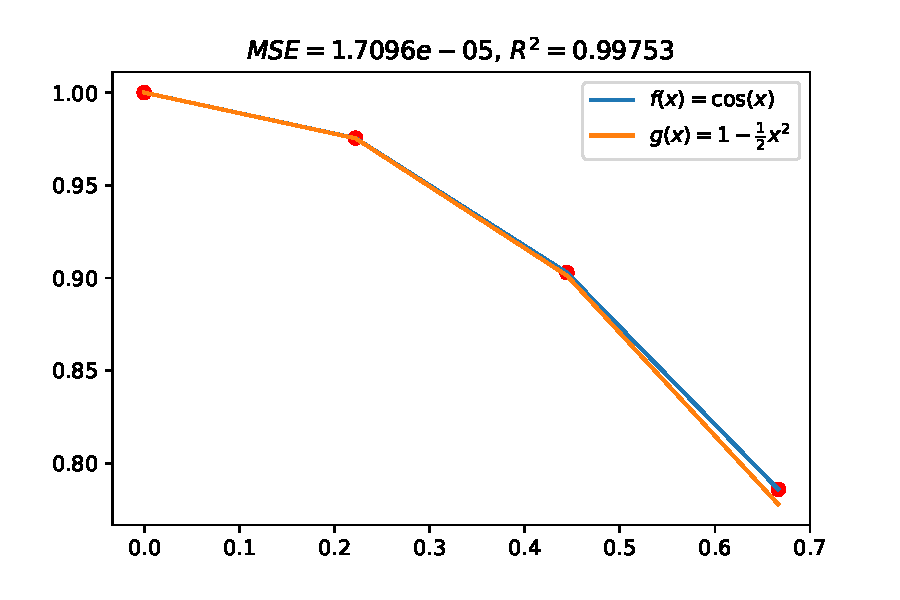
\includegraphics[width=0.9\textwidth]{img/pochi_dati.pdf}
    \caption{Fitting $f(x)=\cos(x)$ with $g(x) = 1-x^2/2$ on the dataset $X = [0, 0.22, 0.44, 0.66].$}
    \label{fig:pochi_dati}
\end{figure}
Imagine the first sampling run from $f(x)$ returns the red points depicted in figure \ref{fig:pochi_dati}; in this example we assume we are sampling points from $X = [0, 2]$ using a deterministic approach, consisting in using a discrete grid that starts from $x = 0$ and contains $n$ points with variable $n$ - so that if $n=4$ the points in \ref{fig:pochi_dati} are obtained. 
With this data it is possible that a machine learning model will learn to approximate $f$ using the function $g(x) = 1 - x^2/2$. According to our dataset this approximation is quite good, as can be seen by inspecting the figure; using quantitative metrics we can confirm this. For example we obtain $\text{MSE} \approx 1.71\vdot 10^{-5}$ and $R^2\approx 99.8\%$, which are basically perfect scores. And yet from basic calculus we know that $\cos(x) \sim 1-x^2/2$ only for $x\sim 0$; indeed if we generate six more samples with slightly larger $x$ values we immediately obtain that $g$ is actually a poor overall approximation of $f$.
\begin{figure}[H]
    \centering
    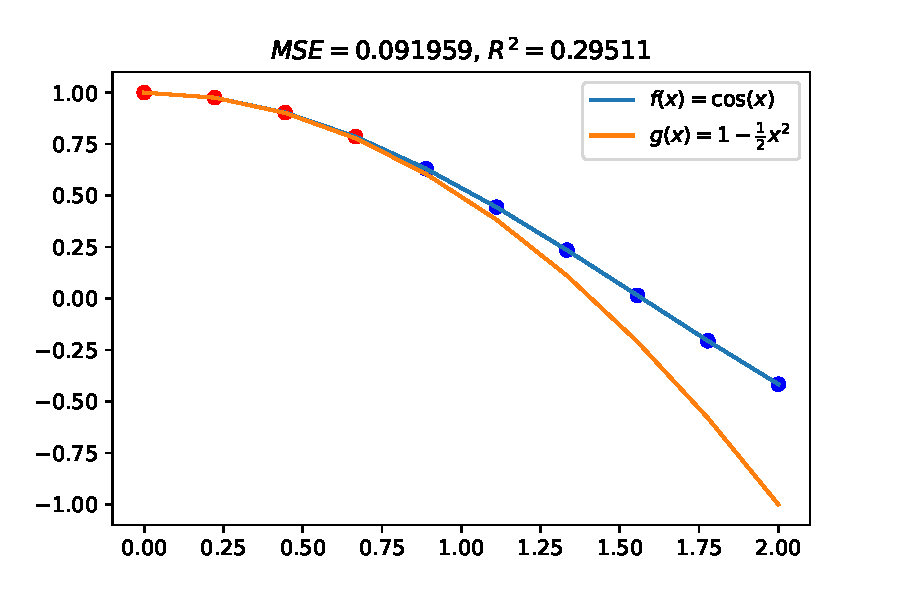
\includegraphics[width=0.9\textwidth]{img/molti_dati.pdf}
    \caption{Fitting $f(x)=\cos(x)$ with $g(x) = 1-x^2/2$ on the dataset of 10 linearly spaced points between $0$ and $2$.}
    \label{fig:molti_dati}
\end{figure}
By adding just a few close-by points (depicted in blue in fig. \ref{fig:molti_dati}) we immediately notice a rapid drop in $g$'s performance, both visually and numerically; in particular the MSE has increased by about $5379$ times ($4$ orders of magnitude), while the $R^2$ has decreased by about $3.4$ times.

Notice that this failure clearly is \emph{not} the model's fault: the dataset it was presented for training was not rich enough. This is the reason why we stated many times that the quality of the dataset is the true limit in all machine learning application: the world's most advanced model cannot do much if the data are too few or too noisy.
In the particular case of this example we notice that increasing $n$ and retraining the model can lead to a much better approximation.

Thanks to this example we can appreciate an important result: even though re-running hyperparameter optimization for longer may have some advantages (as explained above) the only way that is almost guaranteed to increase model performance is \emph{enlarging the dataset}. Indeed if the cause of the model's failure was that it did not observe a large enough population the solution is showing more points to the model.

\paragraph{Representative Samples}
% AGGIUNGERE QUESTIONE DI RAPPRESENTANZA... % We verified that this fraction of parameter samples randomly selected for testing purposes from the training set still represents a homogeneous and uniformly distributed sample for each parameter.
% fai esempio di regressione del compito di NNDL per mostrare come anche se dei dati sono numerosi questo può non bastare
% sistema: tornando su rimpiazza ogni menzione di rappresentatività con semplicemente "abbastanza numerosi", e poi solo dopo spieghi la problematica statistica
The above discussion is slightly imprecise from a statistical point of view; let us briefly fix this.
The important statistical property that, if satisfied by the dataset, ensures good model performance is called \emph{representativeness}. By definition \emph{a representative sample is a subset of a population that seeks to accurately reflect the characteristics of the larger group, i.e. the smaller group is typical of the larger one}. This property should be the true goal, not simply a huge dataset. Indeed imagine that we have a large number of samples, but  a)the available data are all too similar, and b) the true data generating distribution can generate samples that are very different. An example of this is figure \ref{fig:molti_dati}: assuming the true distribution can generate points between $[0, 2]$ a dataset that contains only points in $[0, 0.7]$ (as in fig. \ref{fig:pochi_dati}) will \emph{not} be representative of the true underlying distribution. Indeed even if we had hundreds of points in the $[0, 0.7]$ interval but none in $[0.7, 2]$ the resulting dataset would simply not contain enough information about the true distribution; for this reason even if a model had good performance in $[0, 0.7]$ it would probably be unable to give accurate predictions in $[0.7, 2]$ - and we could not fault it for this; the model has never seen a point in this second interval, so its guesses may not be particularly accurate.\footnote{This statement is a bit drastic; after all the whole point of regression models is to be able to generalize to new, never-before-seen data. In our example (data in $[0, 0.7]$ but not in $[0.7, 2]$) this can be achieved by e.g. providing some data in $[2, 3]$; then a good model will be able to construct accurate interpolations of the missing interval based on its neighbouring ones. An even simpler solution would be to show the model some data in $[0.7, 2]$, of course; the point is that even without direct information about $[0.7, 2]$ by specifying extra information of some other kind accurate indirect guesses can still be easily made.}

If the important property we should look for is representativeness then why should we care about simply the size of the dataset? After all we just gave a simple counterexample were a huge dataset can still lead to poor model performance.
The solution to this apparent conundrum becomes apparent if we consider that, under the right set of conditions, \emph{representativeness and large datasets become equivalent, i.e. a population representative of the underlying distribution can be achieved simply by obtaining enough data points}. To show this it suffices to notice that \emph{if the sampling procedure is unbiased by obtaining enough points the sampled distribution will over time converge to the true underlying distribution}. 
In e.g. the previous example the sampling procedure was chosen exactly because it was \emph{not} unbiased: even though the true distribution is defined over $[0, 2]$ we purposely chose to sample only points in $[0, 0.7]$; since this procedure is biased the sampled distribution will never converge to the true one. If instead the points are sampled from the true distribution without bias, e.g. as in fig. \ref{fig:molti_dati}, over time by the law of large numbers the sampled points will give a better and better approximation of the underlying distribution.

Statistics gives many tools to decide whether a sample is representative (e.g. whether it has enough samples, given the sampling procedure is unbiased), to analyze the relation between true and reconstructed data generating distributions, and so on; discussing them is beyond the scope of this work. 
For our purposes it suffices to notice the following: \emph{to ensure good model performance the user should check that the chosen number of selected samples is large enough that the dataset represents a homogeneous and uniformly distributed sample for each parameter}. For example if we each parameter uniformly from the relevant interval then over time (as long as the number of points is large enough) the resulting sample distribution will cover every part of the relevant region uniformly, i.e. without leaving out any part (which would lead to biases).

To recap: having a large enough dataset can still not be what fixes poor model performance; what we actually should look for is a dataset which is \emph{representative enough}. With the right choice of the sampling algorithm these two conditions (large enough, representative enough) become equivalent; in particular it suffices to ensure that there are no obvious unfair biases\footnote{The asymmetries induced on purpose as in section \ref{subsec:sampling_strategies} are fair.} in the sampling procedure, after which we can forget about representative and only focus on increasing the dataset's size. Still to be safe the user should check that this procedure works in their specific case, i.e. that situations like in figure \ref{fig:molti_dati} are avoided.

\paragraph{Increased Data Generation vs Further HP Optimization}
To recap the previous paragraphs: performing more trials with the same dataset may sometimes fix the issue of poor performance, but if the cause of this failure is that the dataset is inadequate the only way to address the problem is to increase the dataset's size.

This poses a new problem: in the context of plausible scenarios where \textsc{CosmoLIME} may be applied generating new data is expensive. That this holds is almost guaranteed, as accelerating expensive functions evaluations is exactly the reason why emulators are used. Assume for example that generating new samples takes 20 times more CPU time than it takes to do an \texttt{optuna} run; in this case it seems reasonable enough to at least \emph{try} the ``more \texttt{optuna} trials'' approach before yielding to the ``more data'' approach as a last resort. If instead model training is the pipeline bottleneck (which can happen if the model is super complex, for example) then more data should probably be generated with generosity every \texttt{component} iteration.
We remark that solving this issue is of paramount importance: as we showed generating new data is both the preferred solution to unsatisfactory performance and a potentially expensive way to proceed. The other possible approach is performing more \texttt{optuna} trials, which while often cheaper is also not often capable of actually improving the situation.

Since which approach is more efficient in practice clearly depends on the problem at hand (and in particular on the time it takes to generate data compared to the training of new models) it becomes evident that there is no universal way to choose how often to generate new data. 
The way \textsc{CosmoLIME} deals with this issue is therefore by leaving this up to the user,\footnote{As shown above a good criterion to choose how often generate/train is to use the ratio between the average times required by these two operations. These times can usually be easily estimated by comparing the complexity of the machine learning model with that of the numerical code computing $f(x)$; the user's prior knowledge about the problem can often be enough to determine this. In case it is not one can just as easily perform some tests, e.g. by measuring the CPU time needed to perform a typical model optimization or $f$ evaluation.} similarly to what had to be done in the case of the data sampling strategy (sec. \ref{subsec:sampling_strategies}). In particular one of the user-provided parameters that \textsc{CosmoLIME}'s parser will pass to \texttt{component} is \emph{the number of epochs between consecutive generations} (which we can call $N_g$), i.e. the number of times \texttt{component} should retry optimizing the hyperparameters before resorting to asking \texttt{generator} to compute new data points. Using this parameter \texttt{component} only has to perform these steps:
\begin{itemize}
    \item Try to generate data once and optimize the model using them; if the target accuracy is achieved stop execution.
    \item If the threshold has not been reached run again the hyperparameter optimization procedure \emph{with the same} \texttt{optimizer} until $N_g$ iterations have passed.
    \item When $N_g$ epochs have passed generate a new dataset, consisting of the old one plus new samples. Then \emph{reset the} \texttt{optimizer} (i.e. clear \texttt{optuna} history) and go back to the previous step.
    \item Continue this alternation between \emph{data generation phases} and \emph{model training phases} until the target threshold or the max. number of allowed iterations is reached.
\end{itemize}
Notice that the \texttt{optimizer} \emph{must} be reset if a new dataset is produced; as we have seen in the simple cosine example with bad training data the learned information can be misleading when choosing the model, so it is best to start from scratch. Even in situation where the original dataset was not bad but just not good enough we should reset the \texttt{optimizer}: models trained with more data have a natural advantage, therefore they are expected to have improved accuracies, making the comparison with the earlier attempts unfair. Due to this putting scores pertaining to models trained with different data in the same table has no meaning; since this benchmark table is exactly the main \texttt{optuna} output we have to ensure its consistency when modifying the conditions under which its values were computed.

Another point is that parametrizing \textsc{CosmoLIME} with $N_g$ implicitly assumes that data generation is more expensive than hyperparameter optimization; if $N_g$ is defined as above new data are generated less often than new \texttt{optuna} trials are performed. As discussed even though this asymmetry can also go the other way (especially in the case of very complex models) since data generation is often more expensive it makes sense to choose this particular parametrization.
\texttt{component} is still compatible with the opposite situation, of course; it suffices to set the input parameters in such a way that $N_g=0$ (if no model training epoch passes between consecutive data generations it means that new samples are obtained after every unsuccessful optimization), and that the number of samples computed per generation is very high (i.e. data generation is generous).

The final remark about \texttt{component}'s algorithm is that this class accepts two input arguments stating how many new samples should be computed during the data generation phase: one for the very first generation (performed before any optimization takes place), and one for all the following ones; we may call these two values $n_0$ and $n$, respectively.
This parametrization is chosen so that a good compromise may be found in situations where data generation is expensive. Indeed if we choose a large $n_0$ and a small $n$ we can compute a large and expensive batch of samples at the beginning, then increase it gradually with lighter computations. This represents a more conservative approach, i.e. a compromise with the ``generous'' data generating strategy.

Having understood \emph{when} \texttt{component} asks \texttt{generator} for new samples the only remaining thing is to address is \emph{how} this request actually takes place.

\subsubsection{Caching Generated Data For The Other Components}
% riprendere quel discorso
We discussed several times (e.g. in sections \ref{subsec:software_hierarchy}, \ref{subsec:data_components_generator} and \ref{subsec:data_components_component}) that a single \texttt{generator} instance can correspond to several \texttt{component} instances and vice versa. Having gained a better understanding about the ``parallel generation, sequential training'' approach taken by \textsc{CosmoLIME} we now briefly revisit section \ref{subsec:data_components_generator} fully taking into account the connection between \texttt{generator} and \texttt{component}; in particular we can now better appreciate why \texttt{generator} is capable of setting aside data related to other components. 
The \texttt{component} loop modifies only one component model at a time; this means that for example when training the first component the requests made to \texttt{generator} are done in order to improve the performance of the first model specifically. As discussed every time data about the first component is generated e.g. via \texttt{camb} the output of this operation actually contains data about every other component, too; in a sense it is impossible to generate data about a single component at a time. This extra data is unnecessary when it comes to training e.g. the first component, but should not be wasted: indeed by setting it aside we can save it for later. Then when the time to train the other components comes they will find more samples than $n_0$, i.e. the number of points computed in the first run of the generation algorithm; using this approach, i.e. by putting data useful for the future aside, we can improve \texttt{CosmoLIME}'s efficiency. Indeed imagine that for example we have two components, which respectively need 200 and 300 samples to be successfully trained; let us also suppose that $n_0 = n = 100$. Then the first batch will contain 100 samples, and by performing a single request the first component will be successfully trained; when the second component's optimization begins it starts with 200 samples already present, instead of the 100 that were supposed to be. This means that the second component only needs to perform a single request. Had we discarded the ``useless'' second component data while training the first \textsc{CosmoLIME} would have needed to perform three data requests instead of two.

To recap: since model training is sequential (in order to avoid running out of computational resources) it seems that data pertaining to components not currently being trained should be discarded to save memory; by setting it aside, though, we can avoid performing wasteful data generation requests in the future, as those extra requests would ask for exactly the data that we are saving. Since the typical data used in cosmological emulation is comprised of simple, relatively small real matrices it follows that the cost of keeping this extra data samples in memory is negligible; in the event it is not (i.e. the data is so large that it can block the memory needed to perform hyperparameter optimization) the extra data can be offloaded to disk. This slows down everything, but is still beneficial as \texttt{generator} calls often are the most expensive operation in the whole algorithm.

\subsubsection{Ensuring \texttt{generator} Provides New Samples}
% parla di seed
To conclude this part we revisit the discussion contained towards the end of section \ref{subsubsec:prior_knowledge_generator}. 
Assuming the user-defined function passed to \texttt{generator} uses random sampling to pick where to evaluate the target function $f$ it makes sense to ask the user to include a \texttt{seed} parameter, to ensure reproducibility. Another reason why enforcing a \texttt{seed} argument is that we can use it to ensure that the same \texttt{generator} is capable of returning different data samples; as discussed in the previous sections expanding the dataset can fix unsatisfactory model performance, but of course this hinges on having new, independent samples.
In order to comply with the need to alternate between data generation and model training phases \texttt{component} has an internal counter that keeps count of the current iteration (i.e. it starts from 0, then increases to 1, then 2 and so on); it seems only natural to design \texttt{component} in such a way that this counter is also used to update the \texttt{seed} parameter to be used to request new data from \texttt{generator}.\footnote{Of course infinitely many other choices are possible; the only thing that matters is having a sequence of different numbers. Since \texttt{component} needs to count from 0 upwards anyway this sequence naturally appears inside the class, and therefore using it is the most obvious thing to do.}
We argue that this approach (enforcing a mandatory \texttt{seed} argument that is used to enlarge the dataset) naturally extends to cases where the user-provided generating function employs a deterministic sampling scheme (e.g. grid-based). Indeed as said above the main purpose the \texttt{seed} parameter serves is to increase the size of the dataset; this same goal can be achieved in this second case by having \texttt{seed} be a measure of the ``richness'' of the deterministic sampling. For example if the sampler uses a grid \texttt{seed} can measure its coarseness, i.e. increasing the seed corresponds to a finer grid and therefore to more samples. Using this approach actually means that the number of samples that must be computed scales \emph{multiplicatively}, which can exponentially increase the cost of the sampling; but since the old data are not discarded in order to obtain a finer grid what suffices to do is to use the \texttt{seed} to define an offset of the same grid. In this way the scaling is \emph{additive} i.e. linear in the number of generation iterations.

To recap: the generating function that the user must write must have a signature accepting mandatory \texttt{size} and \texttt{seed} parameters - with other hyperparameters being optional.
In general the only purpose \texttt{seed} \emph{must} achieve inside the user-defined generating function is to \emph{vary the returned outputs}. This is necessary because this function is not supposed to accept a certain number $N$ of $x$ values and return the $N$ corresponding $f(x)$, but rather to \emph{pick} $N$ $x$ points autonomously and then return the $N$ $f(x)$ values; having a mandatory \texttt{seed} parameter ensures that calling \texttt{generator} repeatedly with the same $N$ always returns different samples.
The other purpose \texttt{seed} serves is ensuring reproducibility, but that is only nontrivial in the case of random samplers and in general can be easily achieved.

Finally notice that \texttt{size} is simply the argument expressing how many $(x, f(x))$ pairs are to be returned i.e. $N$ in the previous discussion.

\section{Emulator}
% emulator: recap di tutte cose + magari i dettagli ad es. sul punteggio, una rappresentazione dell'algoritmo, eccetera
% nel recap puoi dire: generator è il blocco che fornisce nuovi dati quando gli viene chiesto, preprocessing ovvio, optimizer è quello che fissati i dati cerca i migliori iperparametri, component gestisce l'alternanza fra generator e optimizer, emulator mette tutto insieme.
As discussed in section \ref{subsec:common_design_rules} one of the design principle used to write each of \textsc{CosmoLIME}'s blocks is \emph{independence}: each class works can be used independently of the others, i.e. it can be ``exported'' and manually used separately. Having said that the intended use-case is still the one where all the classes are used in conjunction, according to the rules explained in this chapter. It would be unnecessarily cumbersome to force the user to manually instantiate and attach the different blocks; to avoid this the \texttt{emulator} class has been designed.

The \texttt{emulator} class does nothing more than automatically creating one or more instances of the other classes, as needed. In particular the user can provide a single large \texttt{python dict}; \texttt{emulator} will use \textsc{CosmoLIME}'s parser to dispatch every piece of this dictionary where needed (e.g. the generating function to \texttt{generator}, the model architecture to \texttt{optimizer}, and so on), then provide the user with a single method capable of training everything as needed. This ensures the user only has to write a large but guided set of input parameters; we note that in order to do at least some high-level knowledge about \texttt{CosmoLIME} is required (for example why the \texttt{generator} needs to be provided a function requiring \texttt{size} and \texttt{seed} arguments, etc.). This knowledge can be gained via \textsc{CosmoLIME}'s example \texttt{jupyter notebooks}, which summarize the main points of the present work while diving deeper in the technical details of how \textsc{CosmoLIME}'s internal code and the API work.

A full list of \textsc{CosmoLIME}'s required input arguments can be found in the appendix code \ref{code:cosmolime_args_pseudocode}. 
% We also notice that in the case of multiple components \texttt{emulator} allows the user to specify both individual and shared settings (e.g. about the threshold accuracies).

To conclude the chapter we briefly summarize its content by reviewing the role of each \textsc{CosmoLIME} piece.
\begin{itemize}
    \item \texttt{generator} takes a user-provided function containing the logic needed to sample as many $x$ points as needed, and the code needed to compute the corresponding $f(x)$ outputs. \texttt{generator} is able to share and put aside generated data in an automated, context-dependent way. A full discussion about these \emph{data components} and one regarding data sampling strategies has been presented.
    \item \texttt{preprocessing} transforms the generated data according to transformations picked by the users; default and recommended options are available, and have been presented in the relevant section. \texttt{preprocessing} is also ``exportable'', i.e. it can be used separately to obtain in conjunction with the final model to compute predictions in inference pipelines. This is necessary, because a model trained e.g. on the normalized version of a certain variable will always expect future values of that variable to be normalized in the same way; since ideally in practical application only the final emulator is shared/published the original dataset is discarded, and therefore cannot be used to re-obtain the preprocessing hyperparameters (e.g. the vectors to subtract from the variable to achieve zero mean). For this reason the only reasonable alternative is to have an exportable \texttt{preprocessing} class, which is the case in \textsc{CosmoLIME}.
    \item \texttt{optimizer} performs the optimization of a machine learning model's hyperparameters using data provided by \texttt{generator} and the Bayesian-inspired, highly optimized algorithms in the open source \texttt{optuna} optuna software framework. In order to achieve this a custom wrapper has been implemented and discussed, which can be used to turn \texttt{optuna}'s API from \emph{imperative} to \emph{declarative}, which has the advantage of abstracting all the internal, low-level details. Thanks in particular to \emph{functional programming} it becomes possible to easily separate the code that must be written by the developer from those written by the user, which ensures they both need to invest minimal effort into using \textsc{CosmoLIME} .
    \item \texttt{component} manages the communication between \texttt{generator} and a pair of \texttt{preprocessing/optimizer} instances. It does so by alternating between \emph{data generation phases} and \emph{hyperparameters optimization phases}; the logic that can be used to minimize the overall computational cost, which hinges on a delicate balance between \texttt{generator} and \texttt{optimizer} calls.
    \texttt{emulator} is the definitive \textsc{CosmoLIME} class. It allows the user to automatically create the needed instances of the other classes; using a powerful parser \texttt{emulator} only needs to receive a long \texttt{python dict}, containing all the relevant user-provided information (for example the ranges from which allowed hyperparameters values are to be sampled).
\end{itemize}

A pictorial version of the above summary was already contained in figure \ref{fig:cosmolime_schematics}, located at the start of this chapter; by ending the chapter with the same summary we have come full circle. By noting this funny coincidence the complete description of \textsc{CosmoLIME}'s inner workings is complete.